% ! TeX root = ../../main.tex
\chapter{Background e contesto}
%
\section{Sostenibilità ed Ecosostenibilità}
\subsection{Definizione}
\begin{description}
    \itemsep1em
    \item [Sostenibilità] viene definita dall'enciclopedia Treccani \cite{treccaniEnc} come, \enquote{\textit{Nelle scienze ambientali ed economiche, condizione di uno sviluppo in grado di assicurare il soddisfacimento dei bisogni della generazione presente senza compromettere la possibilità delle generazioni future di realizzare i propri}}.
    \item [Ecosostenibilità] consiste nell'impostazione delle attività umane senza compromettere gli equilibri della biosfera terrestre e facendo in modo che il consumo delle risorse utilizzato dalla generazione corrente permetta alle generazioni future di averne la stessa quantità.
\end{description}
\newpage
\subsection{Millenium Declaration e Agenda 2030}
Nel settembre degli anni 2000 venne adottata la Dichiarazione del Millennio delle Nazioni Unite (\textit{United Nations Millennium Declaration}) \cite{millennium_declaration} da parte degli stati membri che, considerando alcuni principi considerati fondamentali per le relazioni internazionali nel ventunesimo secolo (libertà, uguaglianza, solidarietà, tolleranza, rispetto per la natura, responsabilità condivisa), identificarono otto obiettivi principali da raggiungere entro il 2015 chiamandoli \textit{Millenium Development Goals} (MDGs); questi comprendevano:
\begin{description}
    \item[Goal 1] Sradicare l'estrema povertà e la fame
    \item[Goal 2] Raggiungere una educazione primaria universale
    \item[Goal 3] Promuovere l'uguaglianza di genere e potenziare le donne
    \item[Goal 4] Ridurre la mortalità infantile
    \item[Goal 5] Migliorare la salute materna
    \item[Goal 6] Combattere HIV/AIDS, Malaria e altre malattie
    \item[Goal 7] Garantire la sostenibilità ambientale
    \item[Goal 8] Instaurare una partnership globale per lo sviluppo
\end{description}

Come proseguimento del \textit{Millenium Declaration} nel 2015 le Nazioni Unite hanno elaborato e sottoscritto un nuovo programma denominato Agenda 2030 \cite{agenda2030}, contenente 169 traguardi raggruppati in 17 Obiettivi per lo Sviluppo Sostenibile (Sdgs, \ref{sec:sdgs}) con il fine di porre una buona base, condivisa da tutti i paesi membri, da cui partire per costruire un mondo sostenibile dal punto di vista ambientale, economico e sociale.
%
Ciascun Stato membro è tenuto a sviluppare una strategia nazionale e a questo proposito l'Italia ha istituito la cabina di regia "Benessere Italia", un organo della Presidenza del Consiglio, che si occupa di coordinare, monitorare, misurare e opportunamente migliorare le politiche applicate dai Ministeri per l'attuazione della Strategia Nazionale di Sviluppo Sostenibile (SNSvS) \cite{SNSvS}.

Si tratta di una sfida globale che richiede il coinvolgimento non solo dei governi degli stati membri ma anche delle componenti della società come imprese private e pubbliche, società civili e operatori della informazione e cultura.

\subsection{ASviS}
Nel 2016 si è formata l'Alleanza Italiana per lo sviluppo Sostenibile (ASviS) \cite{asvis} su iniziativa della fondazione UniPolis e dell'Università di Roma \enquote*{Tor vergata}, con l'obiettivo di diffondere la cultura dello sviluppo sostenibile, facendo accrescere la consapevolezza dell'importanza dell'Agenda 2030. 

L'ASviS (con logo in figura \ref{fig:asvis-logo}) vede a oggi una partecipazione di oltre 300 soggetti che si occupano di tematiche riconducibili agli Obiettivi di Sviluppo Sostenibile; fra gli aderenti alla alleanza vi sono associazioni, enti di diritto pubblico, università (fra queste anche l'Università di Bologna), enti e centri di ricerca pubblici e privati e tante altre organizzazioni della società civile italiana senza scopo di lucro \cite[Aderenti alla ASviS]{aderenti_asvis}.

Nel concreto questa associazione esercita attività di sensibilizzazione, educazione, formazione, informazione e comunicazione, ricerca scientifica, relazioni istituzionali, organizzazione e gestione di attività culturali e infine monitoraggio della posizione del Paese rispetto agli SDGs con la pubblicazione di rapporti annuali.

\begin{figure}
    \center
    
\includegraphics[height=4cm]{img/Logo-ASviS.jpg}
    \caption{Logo di Alleanza Italiana per lo sviluppo Sostenibile (ASviS)}
    \label{fig:asvis-logo}
\end{figure}
%
\subsection{SDGs}
\label{sec:sdgs}
Gli Sdgs (\textit{Sustainable Development Goals})\cite{agenda2030}, in italiano Obiettivi per lo Sviluppo Sostenibile sono obiettivi principali da ambire e raggiungere da ogni stato membro e le sue componenti della società entro il 2030. Imprese private e pubbliche, operatori della informazione e società civili sono coinvolte in questo ambizioso progetto andando ad agire concretamente ad esempio per ridurre le disuguaglianze, sconfiggere la fame, lottare contro il cambiamento climatico e raggiungere una parità di genere.
Di seguito i 17 obiettivi per lo sviluppo sostenibile e le loro grafiche (Figura \ref{fig:sdgs}):
\begin{description}
    \item[Goal 1] Sconfiggere la povertà
    \item[Goal 2] Sconfiggere la fame
    \item[Goal 3] Salute e benessere
    \item[Goal 4] Istruzione di qualità
    \item[Goal 5] Parità di genere
    \item[Goal 6] Acqua pulita e servizi igienico-sanitari
    \item[Goal 7]  Energia pulita e accessibile
    \item[Goal 8] Lavoro dignitoso e crescita economica
    \item[Goal 9]  Imprese, innovazione e infrastrutture
    \item[Goal 10] Ridurre le disuguaglianze
    \item[Goal 11] Città e comunità sostenibili
    \item[Goal 12] Consumo e produzione responsabili
    \item[Goal 13] Lotta contro il cambiamento climatico
    \item[Goal 14] Vita sott’acqua
    \item[Goal 15] Vita sulla Terra
    \item[Goal 16] Pace, giustizia e istituzioni solide
    \item[Goal 17] \textit{Partnership} per gli obiettivi
\end{description}
%
\begin{figure}
    \centering
    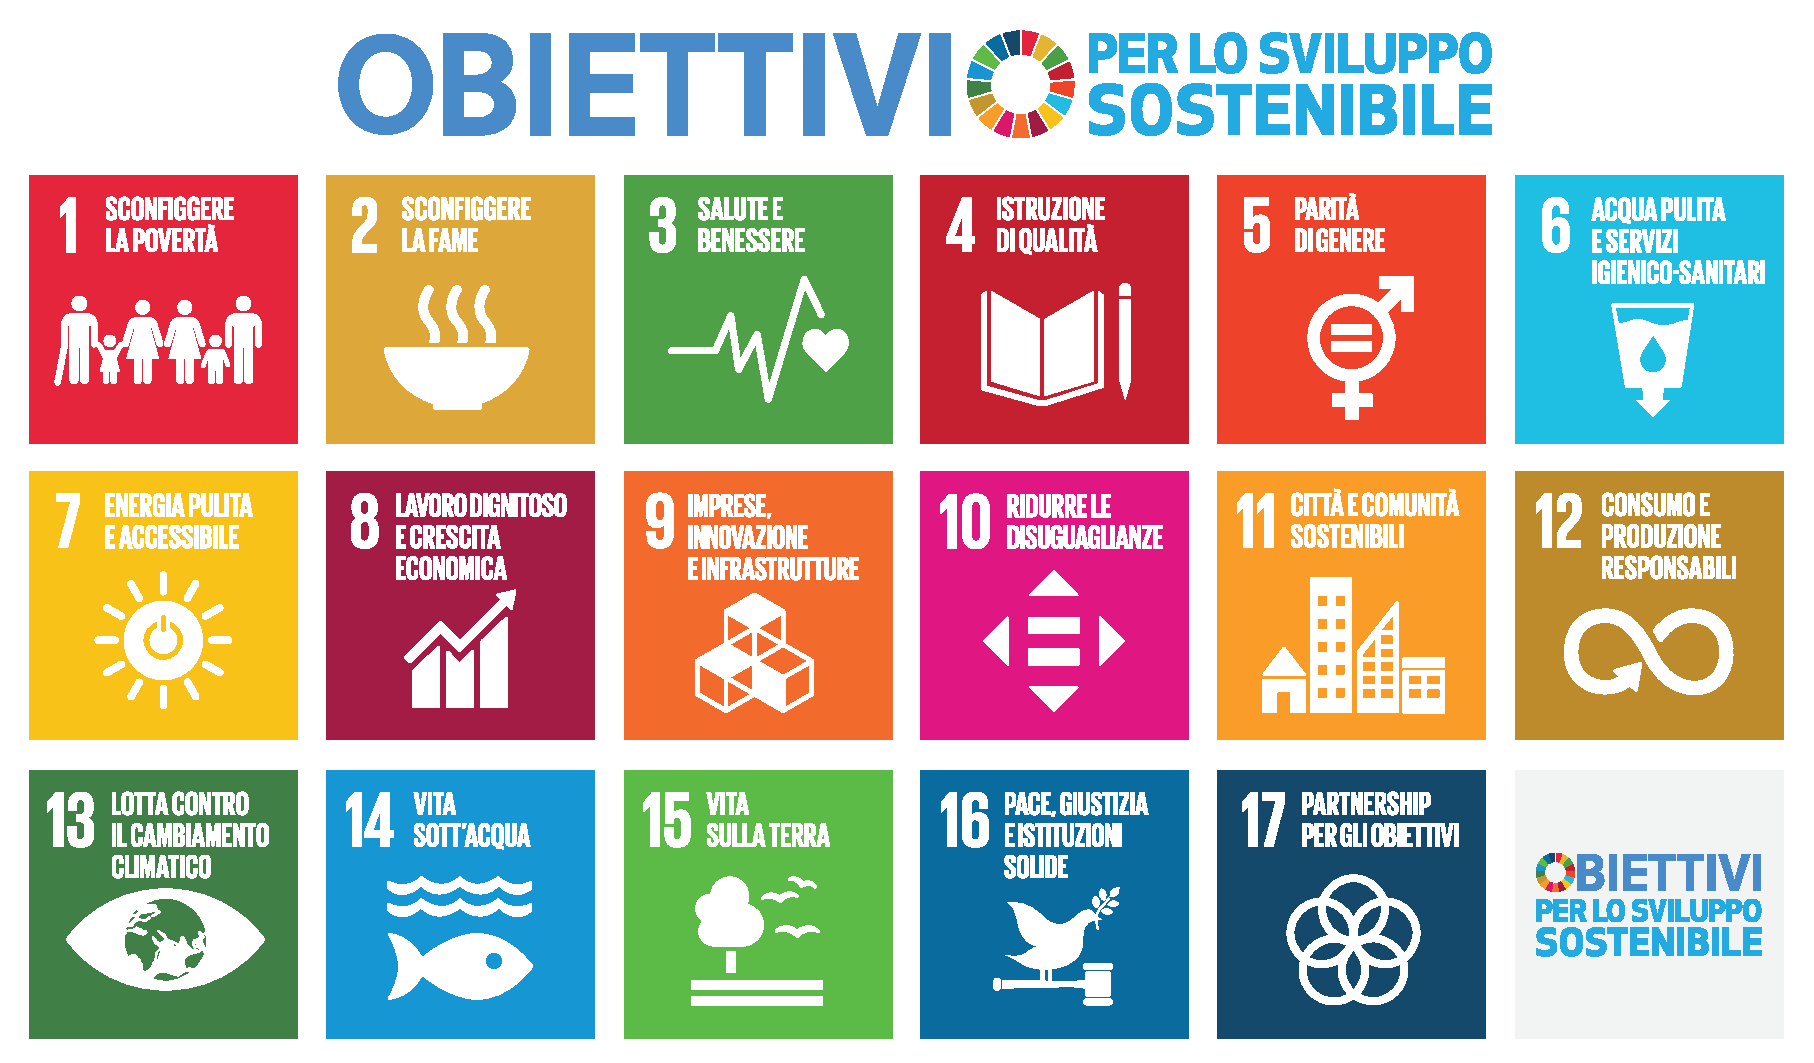
\includegraphics[width=\textwidth]{img/SDG_Poster.png}
    \caption{Grafiche dei 17 Obiettivi per lo sviluppo Sostenibile}
    \label{fig:sdgs}
\end{figure}

\section{Progetto ReMade}

Il progetto ReMade (REplanting for Monitoring Accomplishment of DEmaterialization, \cite{remade_project}), nato con la collaborazione del CESIA, DICAM e DISI Sustainable ICT LAb, fa parte di una serie d'iniziative intraprese dalla Università di Bologna per contribuire al raggiungimento degli Obiettivi per lo Sviluppo Sostenibile.

Lo scopo di questo progetto è quello di potenziare l'effetto del processo di dematerializzazione (riduzione di uso di carta nei processi amministrativi e di comunicazione), traducendo il risparmio di carta nella piantumazione proporzionale di alberi negli spazi verdi e affiancare una \textit{web app} \cite{remadeApp} per diffondere i risultati virtuali (meno carta) e reali (più alberi) al fine di aumentare la consapevolezza da parte della comunità UniBo.

In  questo contesto il contributo di questa tesi mira ad aumentare l'interesse e la consapevolezza sul tema della ecosostenibilità e sul risparmio di carta attraverso l'integrazione di una applicazione per smartphone e un totem multimediale con anche l'aiuto della realtà aumentata e la \textit{gamification}.
\begin{figure}
    \center
    \includegraphics[height=6cm]{img/remade_logo.png}
    \caption{Logo del progetto ReMade}
    \label{fig:remade_logo}
\end{figure}

Con questo progetto l'Ateneo contribuisce a tre degli obiettivi per lo sviluppo sostenibile (Figura \ref{fig:remade_dgs}) che riguardano le città e comunità sostenibili (Goal 11), la lotta contro il cambiamento climatico (Goal 13) e la vita sulla terra (Goal 15); infatti la piantumazione di nuovi alberi porta inevitabilmente a diversi benefici come la riduzione della temperatura, rimozione d'inquinanti atmosferici e miglioramento dello stile di vita e vivibilità delle città.
\begin{figure}
    \centering
    
\includegraphics[width=\textwidth]{img/sdg_remade.png}
    \caption{Obiettivi Agenda 2030 sostenuti dal progetto ReMade}
    \label{fig:remade_dgs}
\end{figure}
\newpage
\section{Motivare gli utenti}
Considerati gli obiettivi del progetto ReMade, al fine di coinvolgere il più possibile la comunità universitaria UniBo, vengono impiegate diverse tecniche come la \textit{Gamification} e l'uso di \textit{Serious games}.
%
%
\subsection{Gamification}
\label{sec:gamification}
Prima di discutere il significato e le implicazioni che il fenomeno della \textit{gamification} sottintende occorre fare una precisazione sui sostantivi inglesi \textit{play} e \textit{game} in quanto assumono sfumature di significato diverso nonostante la loro traduzione in italiano coincida con la parola \enquote{gioco}. Di seguito le definizioni fornite dal \textit{Cambridge Dictionary} \cite{cambridgeDict}:

\begin{description}
    \itemsep1em
    \item [\textit{Play}] \textit{ \enquote*{recreation, amusement}}; attività puramente ricreativa senza regole e obiettivi (es. giocare con giocattoli).
    \item [\textit{Game}] \textit{\enquote*{an activity or sport that people play, usually with rules and needing skill}}; un'attività o sport, dove tipicamente sono presenti regole e sono richieste abilità, il cui scopo è raggiungere uno o più obiettivi (es. giochi da tavolo).
\end{description}

Il termine \textit{gamification} è un termine ombrello informale che indica l'utilizzo di alcuni elementi di gioco (\textit{game elements}) in contesti di tutt'altra natura per migliorare l'esperienza utente (\textit{User Experience UX}) e il suo coinvolgimento \textit{(User Engagement)} \cite{gamificCHI11}.
Al momento non esiste una definizione univoca ma in letteratura ci si riferisce anche alla strategia della gamification con il concetto di \textit{gameful design} che sottolinea lo scopo di progettare un sistema che sia \textit{gamefulness}, quindi ricco di esperienze e qualità riconducibili al \textit{game} grazie ai suoi elementi e meccanismi \cite{definingGamification2011}.

L'utilizzo della gamification ha avuto un grande successo tanto da esserne immersi nella vita di tutti i giorni. Molti negozi o siti (es. Booking, Figura \ref{fig:booking-genius}) a oggi prevedono un programma fedeltà che comprende l'accumulo di punti per ottenere sconti, molte applicazioni e dispositivi fitness (es. Apple Watch \cite{appleWatchGamification}) sfruttano badge (Figura \ref{fig:appleFitnessBadges}), livelli e sfide periodiche per motivare l'utente a fare movimento (\textit{Games for Health})\cite{game4health},nelle campagne di crowdfunding (es. KickStarter) la raccolta fondi assume l'aspetto di un gioco con obiettivi e premi e nelle app di navigazione come in Waze ritroviamo un meccanismo di classifica fra gli utenti che possono accumulare punti guidando (Figura \ref{fig:waze-level}).

\begin{figure}
    \centering
    \subfloat[App Fitness di Apple: schermata con premi e obiettivi]{
        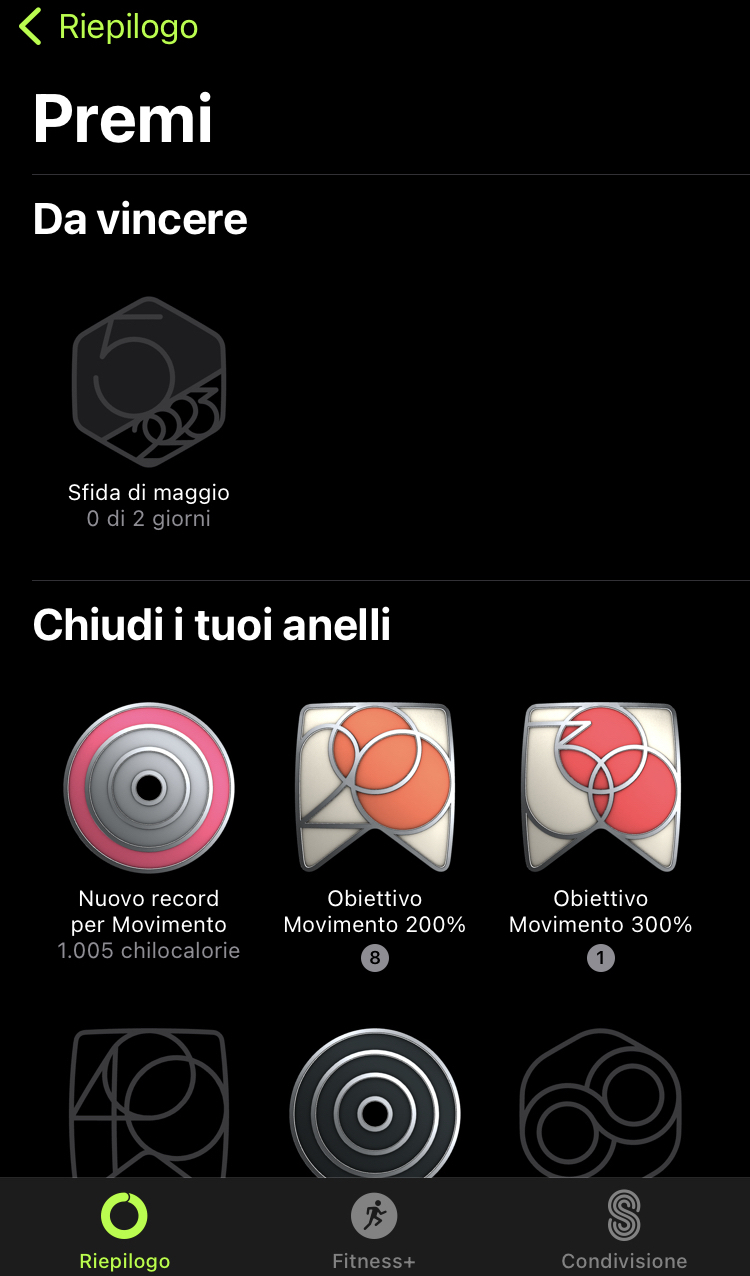
\includegraphics[width=0.4\textwidth]{img/apple-fitness-badge.jpeg}
        \label{fig:appleFitnessBadges}
    }
    \hspace{2em}% Space between image A and B
    \subfloat[Programma fedeltà Genius di Booking: sconti in base al livello]{
        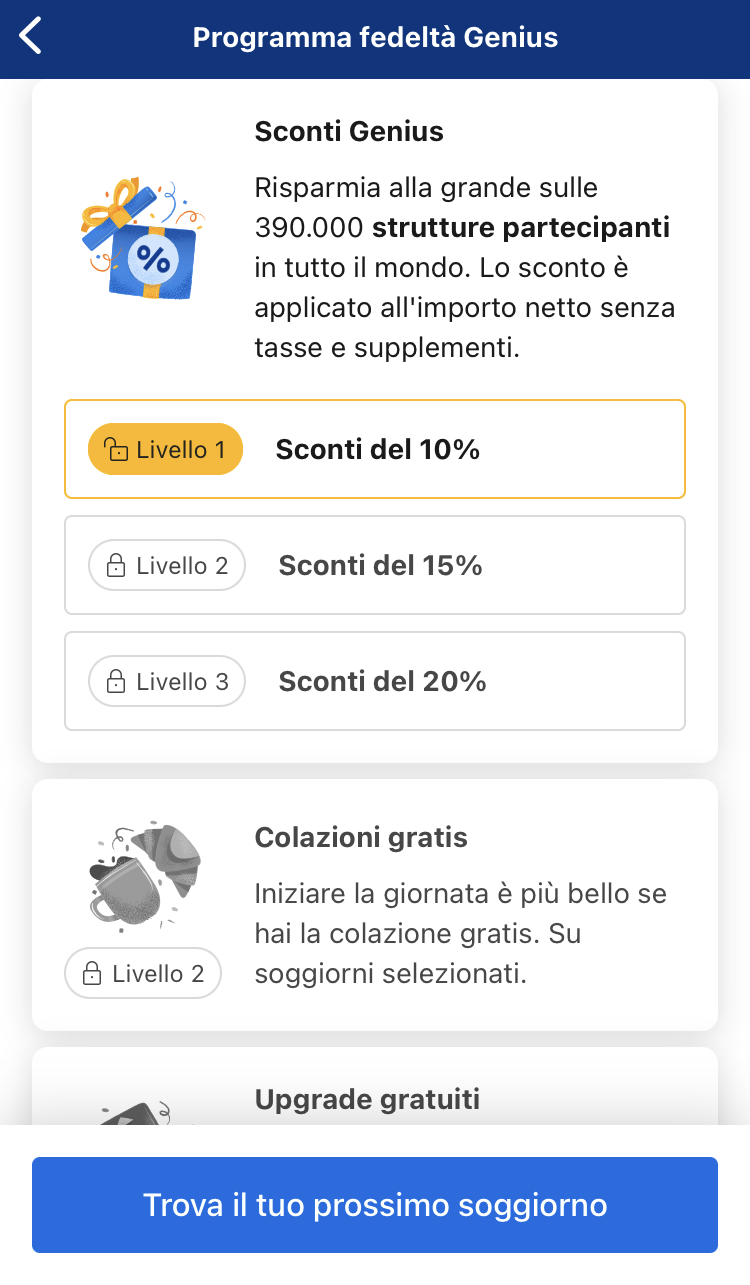
\includegraphics[width=0.4\textwidth]{img/booking-gamification.PNG}
        \label{fig:booking-genius}
    }
    \hspace{2em}% Space between image B and C
    \subfloat[App navigatore stradale Waze: tabellone punti e livello utente]{
        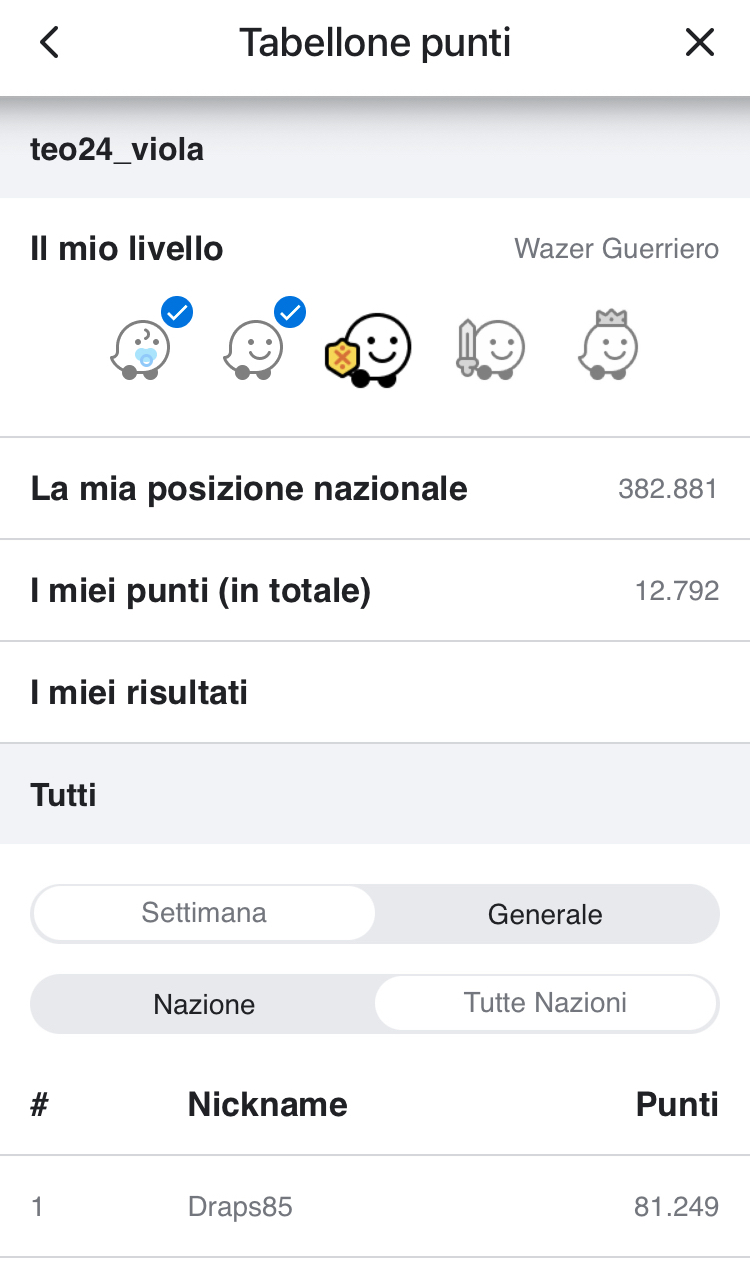
\includegraphics[width=0.4\textwidth]{img/waze2.jpeg}
        \label{fig:waze-level}
    }
    \caption{Esempi di piattaforme e app dove è presente la \textit{gamification}} 
    \label{fig:gamification-example}
\end{figure}

Questo successo è da ricondursi sicuramente alla natura dell'essere umano che ha un costante desiderio di superare sfide, risolvere problemi e ottenere risultati, tutte esperienze che si ritrovano nei giochi, ma anche alle motivazioni che portano l'utente a giocare (motivazione estrinseca e intrinseca \cite{Deci1975IntrinsicMA}), come ad esempio la soddisfazione o la competizione.

I \textit{game elements}, se utilizzati correttamente, fanno leva sulle motivazioni e desideri che portano l'utente a giocare, ottenendo un forte coinvolgimento e intrattenimento.
La definizione di questi elementi non è univoca, di seguito ne vengono presentate due:

\begin{itemize}
    \itemsep1em
    \item la prima è proposta in \citetitle{definingGamification2011}\cite{definingGamification2011} dove vengono identificati cinque elementi su diversi livelli di astrazione:
    \begin{itemize}
        \item \emph{Interface design patterns}: elementi come badge, livelli o classifiche;
        \item \emph{Game design patterns}: per esempio tempo e/o risorse limitate, turni;
        \item \emph{Design principles or heuristics}: gioco duraturo, obiettivi chiari, varietà di stili di gioco;
        \item \emph{Conceptual models of game design units}: modelli concettuali dei componenti o dell'esperienza di gioco;
        \item \emph{Game design methods}: pratiche e processi specifici per la progettazione del gioco.
    \end{itemize}
    %
    \item la seconda invece in \citetitle{Werbach2012ForTW}\cite{Werbach2012ForTW} che vede tre elementi chiave:
    \begin{itemize}
        \item \emph{Components}: tra cui punti, badge, livelli, missioni, classifiche, regali da condividere;
        \item \emph{Mechanics}: comprende i processi che guidano l'azione in avanti e generano coinvolgimento nel giocatore, ad esempio la cooperazione o competizione con altri utenti, turni di gioco, stati di vittoria, ricompense
        \item \emph{Dynamics}: aspetti da considerare e gestire come narrativa, crescita e sviluppo del giocatore, interazioni sociali, emozioni provate durante il gioco
    \end{itemize}
\end{itemize}

Si possono notare in ogni caso delle analogie fra le definizioni, ad esempio gli \textit{interface design patterns} nella prima definizione coincidono con i \textit{components} della seconda.

\subsubsection{Gamification nella educazione}
La \textit{gamification} nel settore educativo ha sempre avuto successo grazie alle qualità che i giochi offrono come scomporre le grandi sfide in passi gestibili, ridurre la paura del fallimento, promuovere il lavoro di squadra o incoraggiare la risoluzione dei problemi, portando a effetti positivi sulla motivazione, impegno e prestazione \cite{gamifEducation}.


Nel caso vengano utilizzati supporti tecnologici si parla di \textit{Plugged Gamification} (es. Kahoot, Duolingo, AR, VR, \dots), altrimenti di \textit{Unplugged Gamification} (es. Quiz, puzzle, gare di teoria a squadre, \dots) \cite{gamificInEducation} ma l'efficacia e la qualità di questi giochi non sono vincolate a questa classificazione, ma dipendono da come sono stati utilizzati i \textit{game elements}.

%
%
\subsection{Serious game}
I \textit{Serious games} sono giochi a tutti gli effetti in quanto utilizzano tutti i \textit{game elements}, sono sviluppati con il principale intento di educare, formare o rafforzare un cambiamento e in secondo luogo intrattenere.

Nella maggior parte dei casi, presentano degli obiettivi chiari e precisi che verranno raggiunti dopo che l'utente avrà imparato qualcosa di nuovo, come può essere un gioco normale, ma vengono utilizzati anche, ad esempio, per formare lavoratori, illustrare o aiutare gli studi di ricerca scientifica, diffondere un messaggio e sensibilizzare, simulare situazioni, pubblicizzare un prodotto o addirittura possono essere utilizzati come trattamento terapeutico.
Di seguito vengono mostrati alcuni esempi concreti di \textit{serious game}.

\subsubsection{Foldit - Ricerca scientifica}
Foldit \cite{foldit} è un gioco unico nel suo genere che permette di manovrare le proteine rappresentate in tre dimensioni permettendo al giocatore di contribuire alla ricerca avanzata sulla salute dell'uomo, alla bioingegneria e biologia. Ogni settimana gli scienziati propongono il problema più recente di ripiegamento di proteine (design delle proteine e di piccole molecole o risoluzione delle strutture).

\begin{figure}
    \centering
    \subfloat[Design di piccole molecole]{
        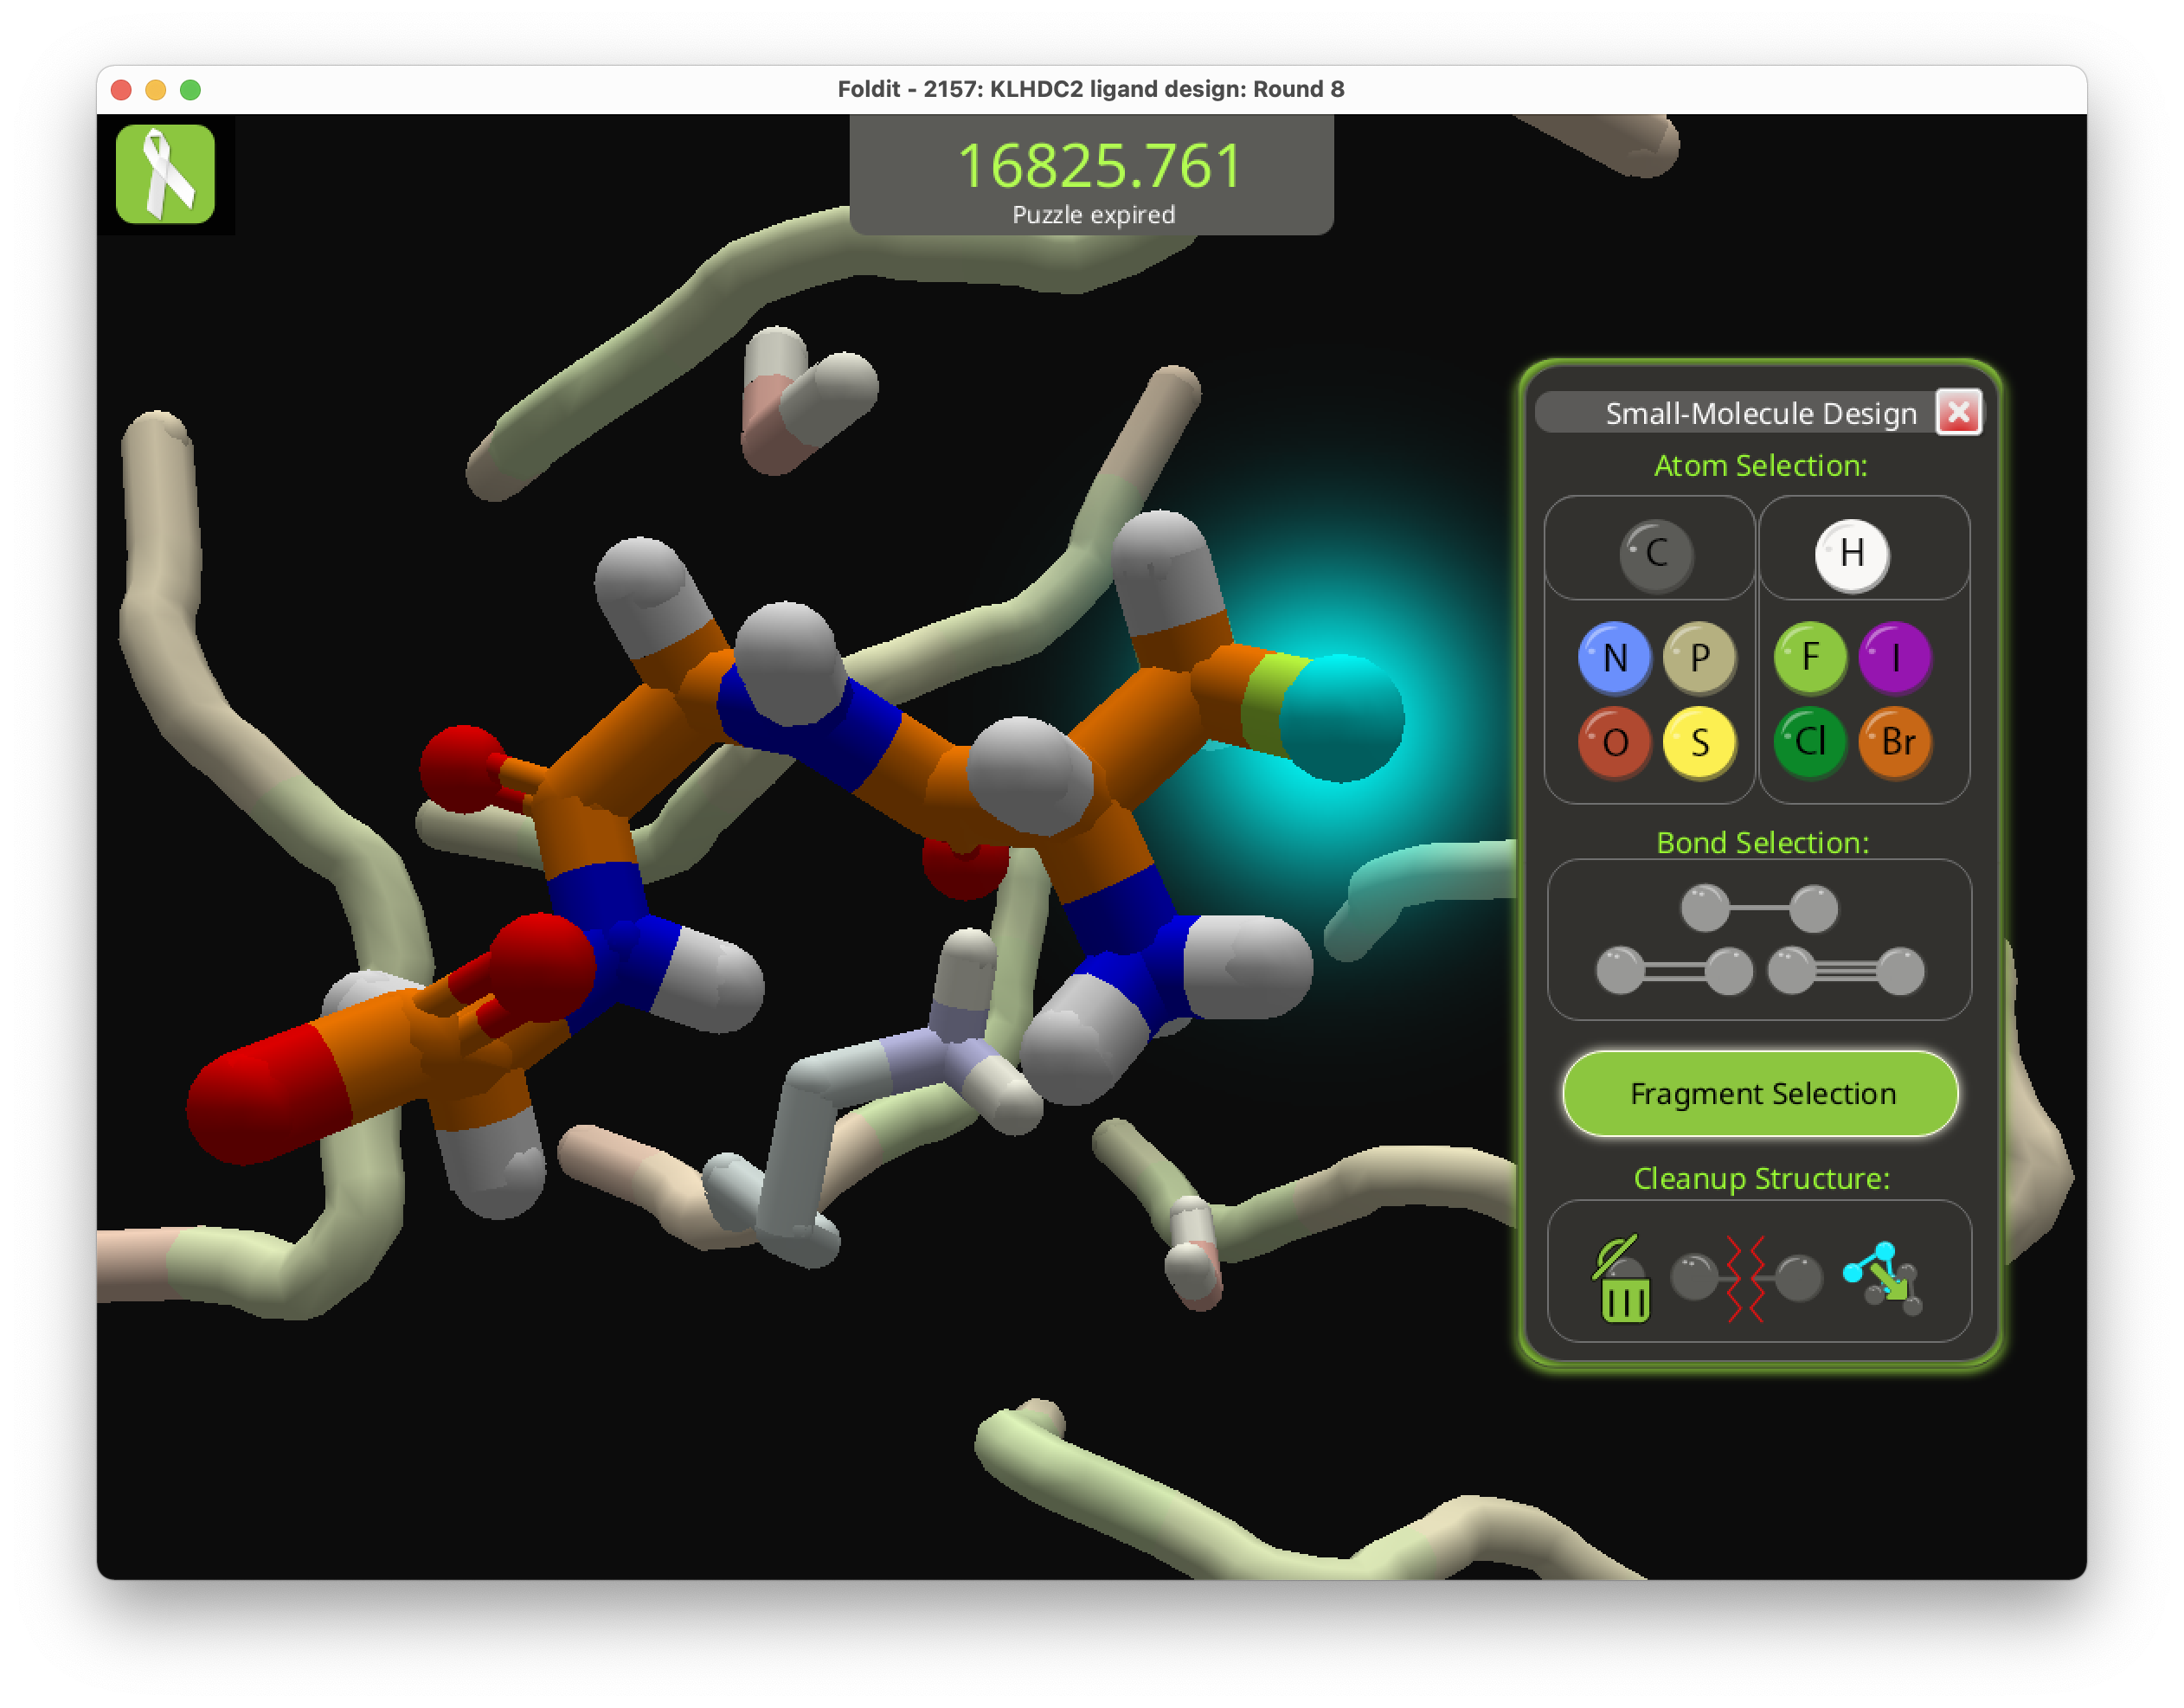
\includegraphics[width=0.45\textwidth]{img/foldit-design.png}
    }
    \subfloat[Risoluzione della struttura delle proteine]{
        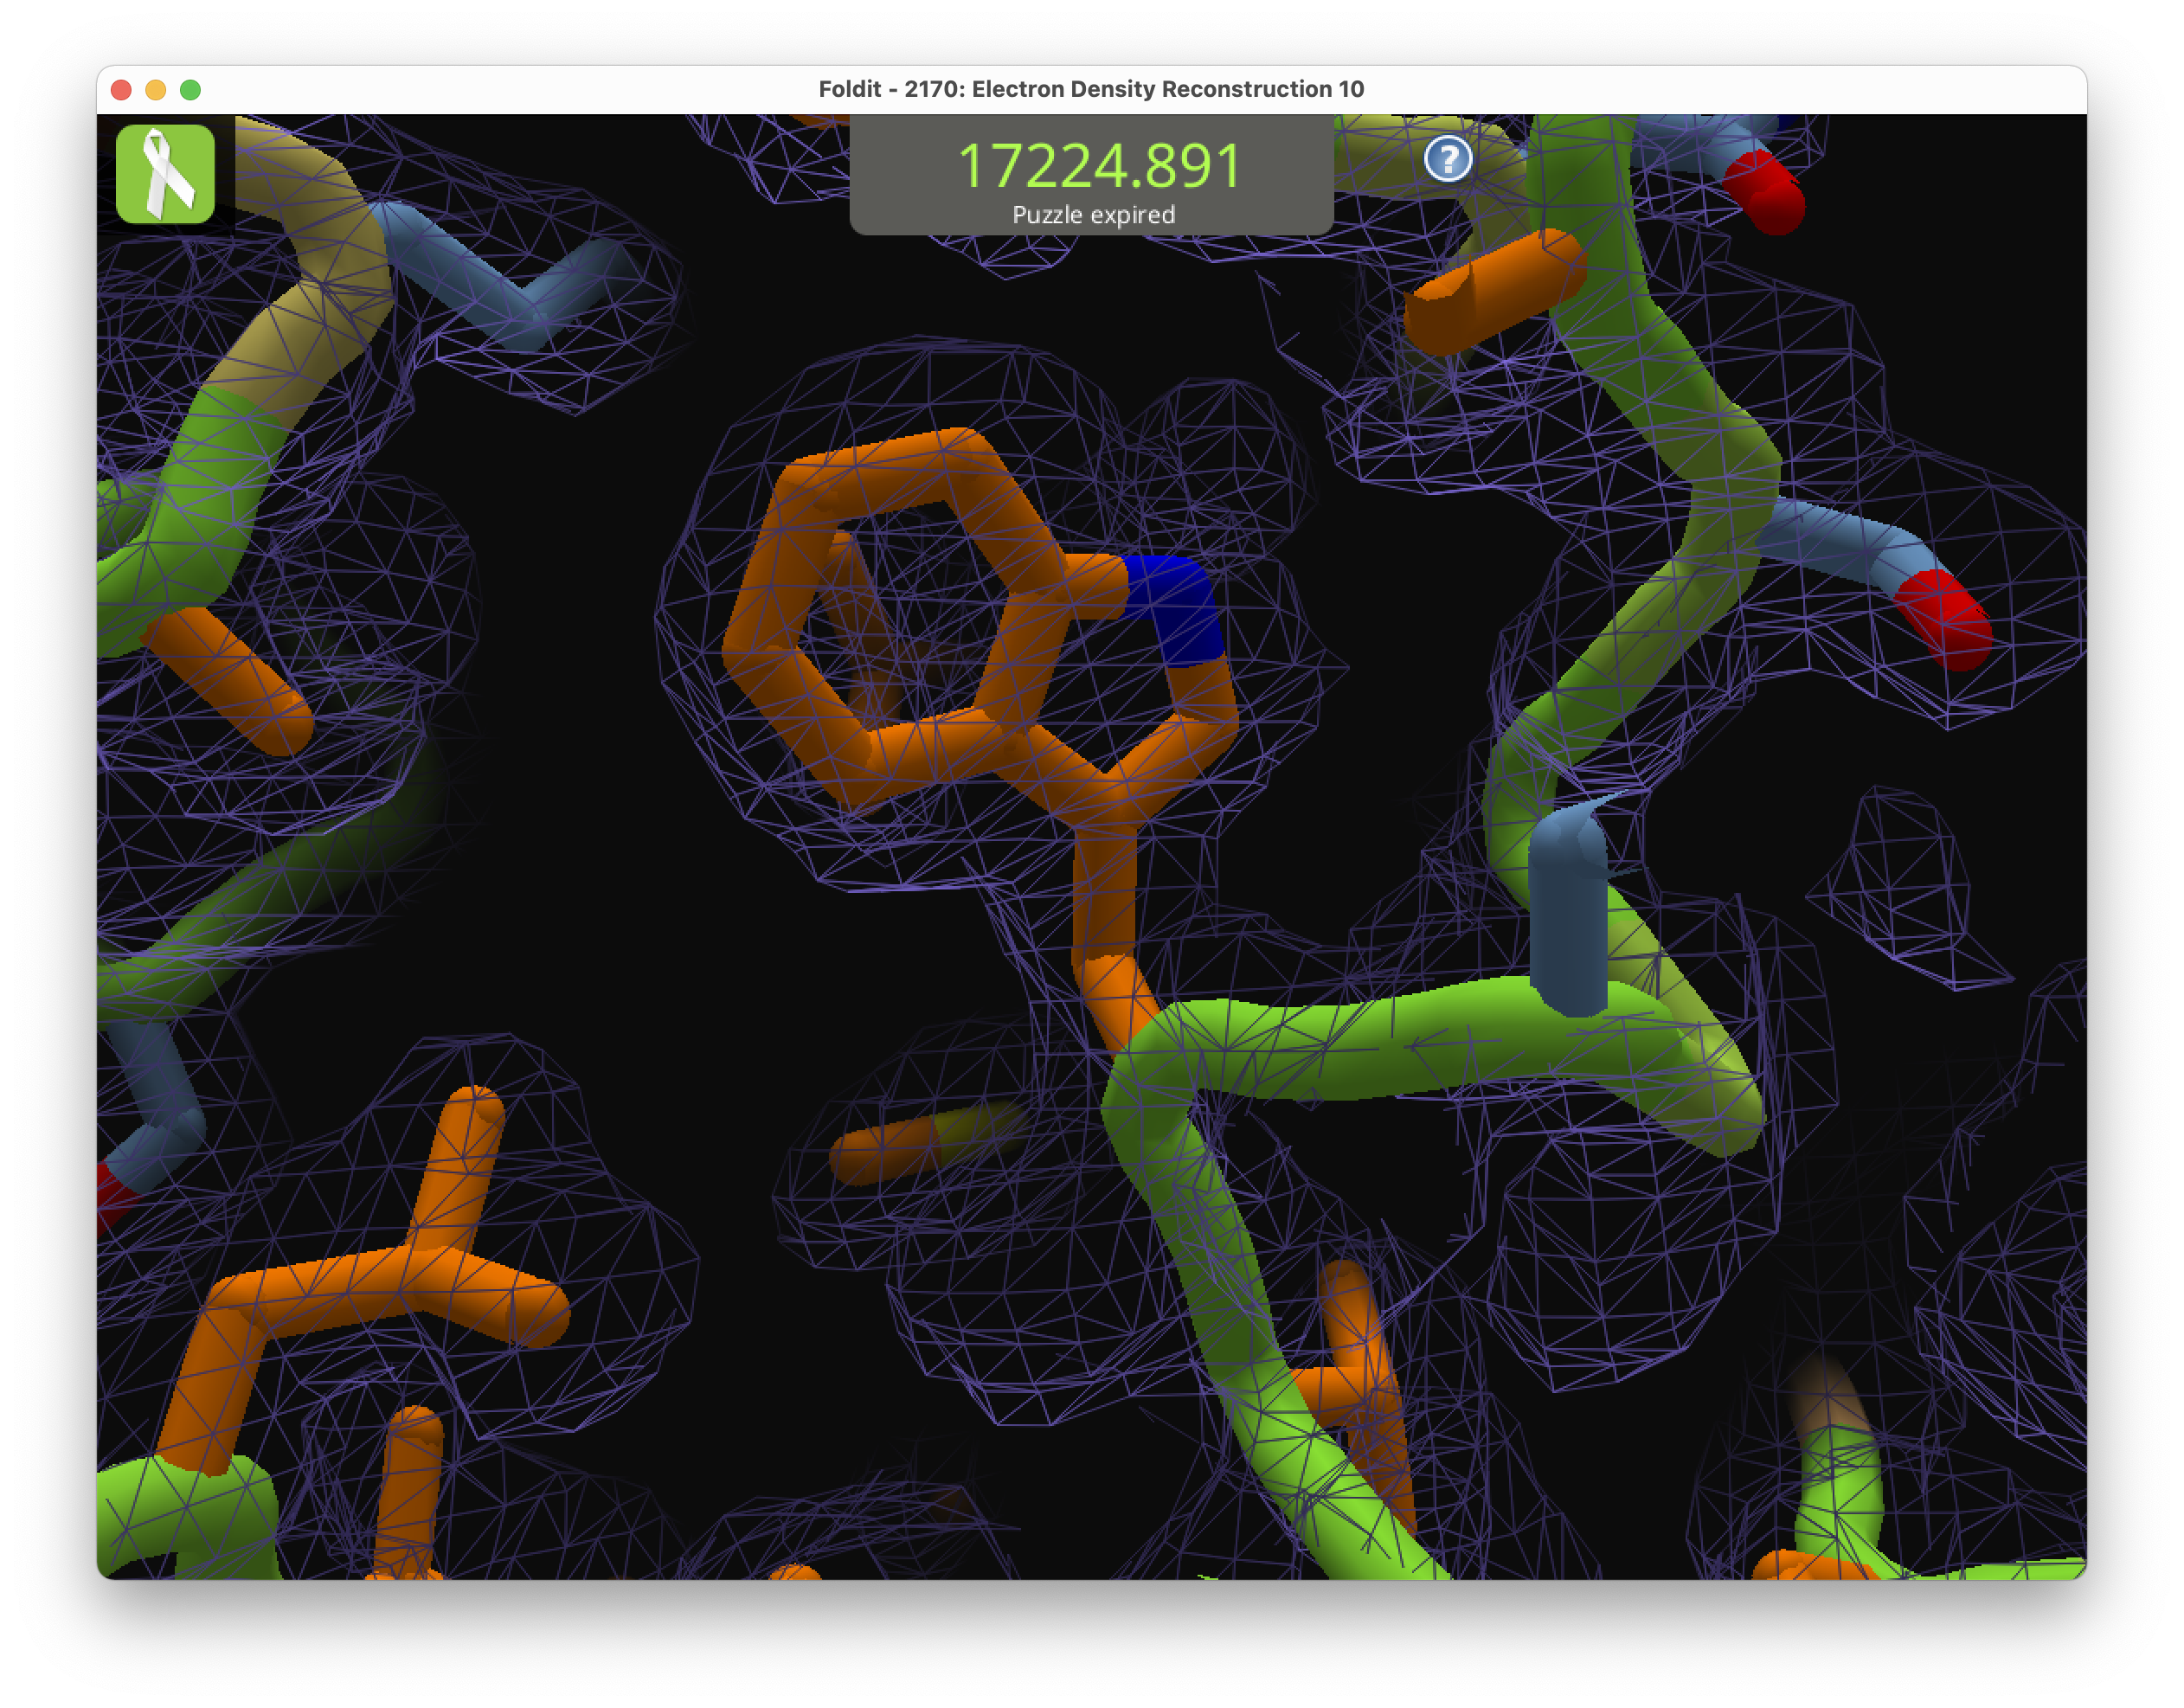
\includegraphics[width=0.45\textwidth]{img/foldit-structure.png}
    }
    \caption{Foldit: serious game per la ricerca scientifica e manipolazione di molecole}
    \label{fig:foldit} 
\end{figure}

\subsubsection{EndeavorRX - Terapia per disturbo da deficit di attenzione}
%todo finire
EndeavorRx \cite{endeavorRx} (Figura \ref{fig:endeavorRx}) è un gioco che aiuta a ridurre il disturbo da deficit di attenzione (ADHD) in bambini di età compresa fra 8 e 12 anni; la FDA (\textit{Food and Drug Administration}) lo ha autorizzato come dispositivo medico e perciò è richiesta la prescrizione medica per l'uso come parte di un programma terapeutico.
\uppercase{è} stato sviluppato dalle migliori menti mondiali di neuroscienza e game designer con lo scopo di agire su parti specifiche del cervello che svolgono un ruolo chiave nella funzione della attenzione.

\begin{figure}
    \center
    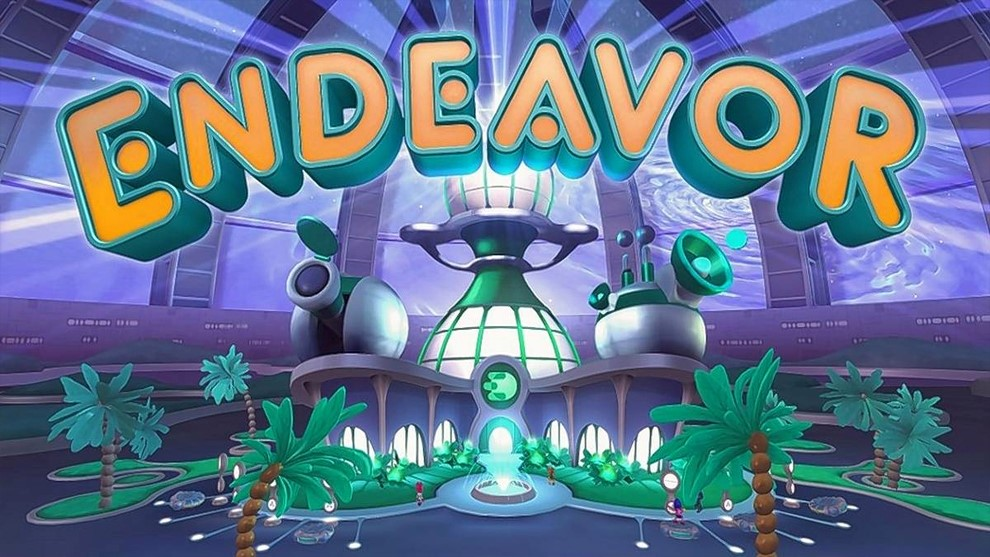
\includegraphics[width=0.5\textwidth]{img/endeavorRx.jpg}
    \caption{EndeavorRx: \textit{serious game} come terapia per disturbo da deficit di attenzione}
    \label{fig:endeavorRx}
\end{figure}


\subsubsection{Dumb Ways to Die - Diffusione di un messaggio}
\textit{Dumb Ways to Die} \cite{dumbwaytodie} (figura \ref{fig:dumbwaytodie}) è un \textit{serious game} promosso dalla Metro Trains Melbourne per promuovere la sicurezza ferroviaria in modo particolare ai più piccoli, veicolando il messaggio attraverso un gioco simpatico e divertente in modo efficace.
\begin{figure}
    \center
    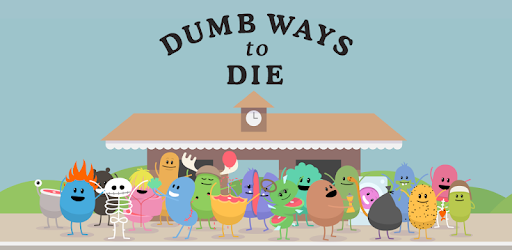
\includegraphics[width=0.5\textwidth]{img/dumb-way-to-die.png}
    \caption{Dumb Ways to Die}
    \label{fig:dumbwaytodie}
\end{figure}

\subsubsection{Information Tower - Educazione}
Information Tower \cite{infoTower} (Figura \ref{fig:infoTower}), finanziato da Google e Altroconsumo, ha l'obiettivo di educare a riconoscere le \textit{fake news} che ogni giorno possiamo incontrare. Vengono forniti tre indizi che permettono di valutare la qualità e la veridicità della notizia, l'utente deve poi dichiarare se quelle proposte dal gioco è un \textit{fake} o è vera. 

\begin{figure}
    \center
    \subfloat[Schermata iniziale]{
        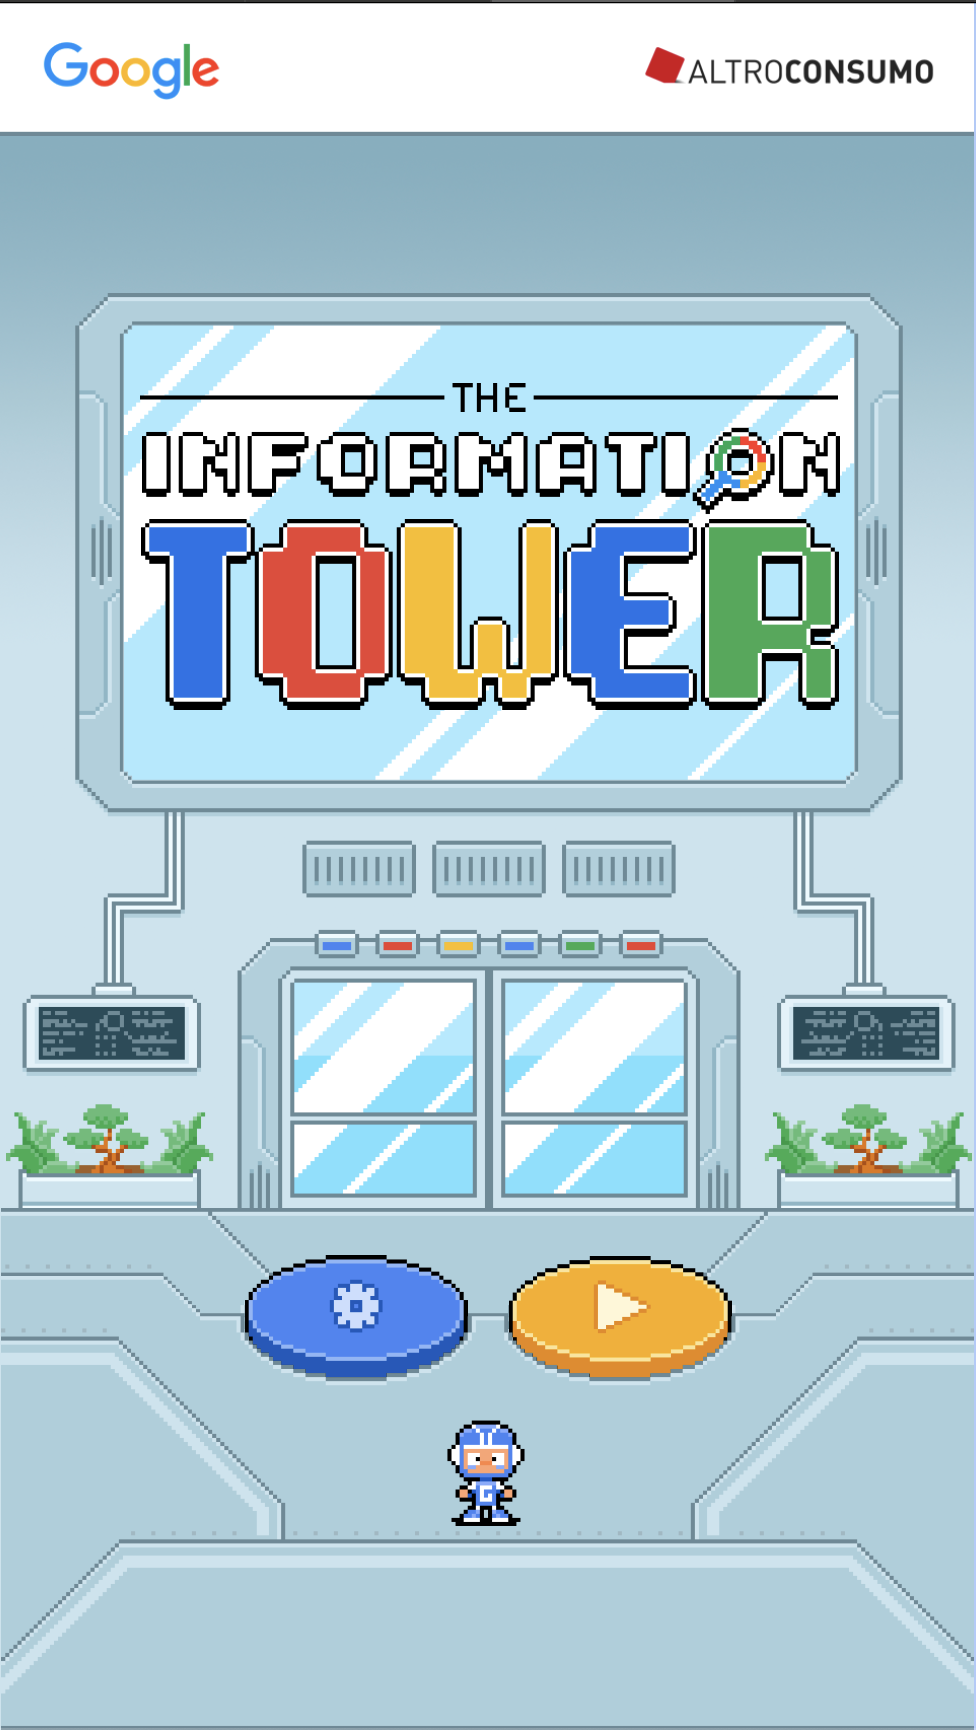
\includegraphics[width=0.30\textwidth]{img/infoTower1.png}
    }
    \subfloat[Lettura fake news, ricerca indizi e riposta]{
        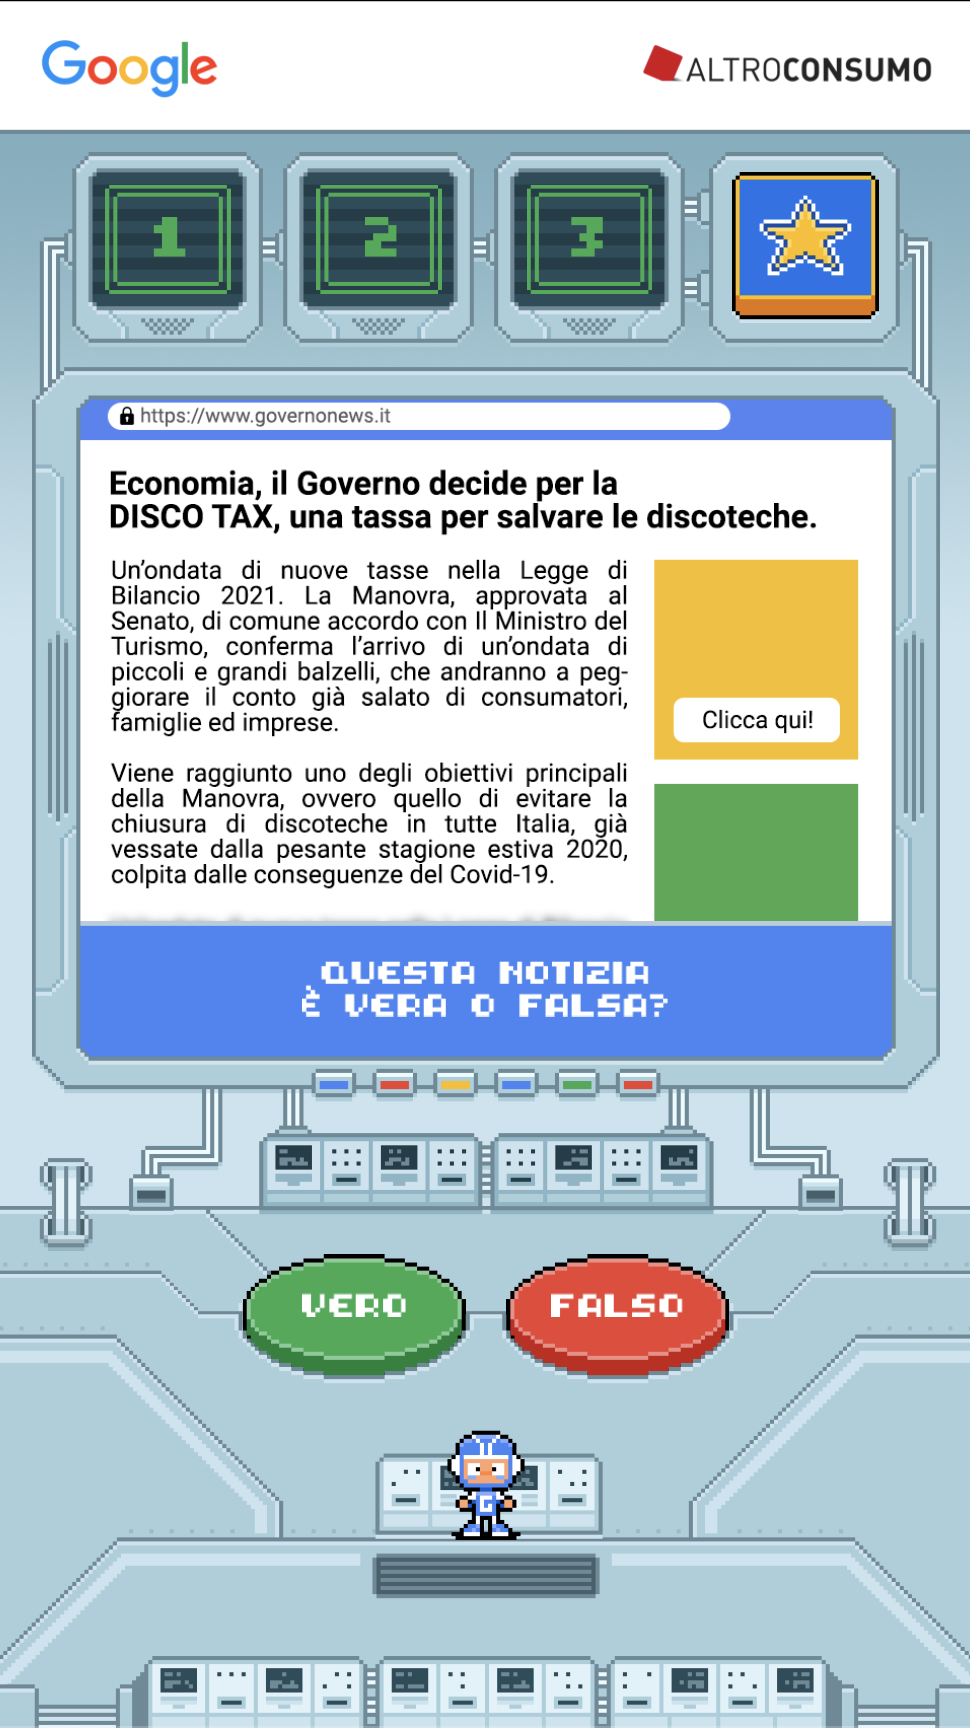
\includegraphics[width=0.30\textwidth]{img/infoTower2.png}
    }
    \subfloat[Schermata superamento livello]{
        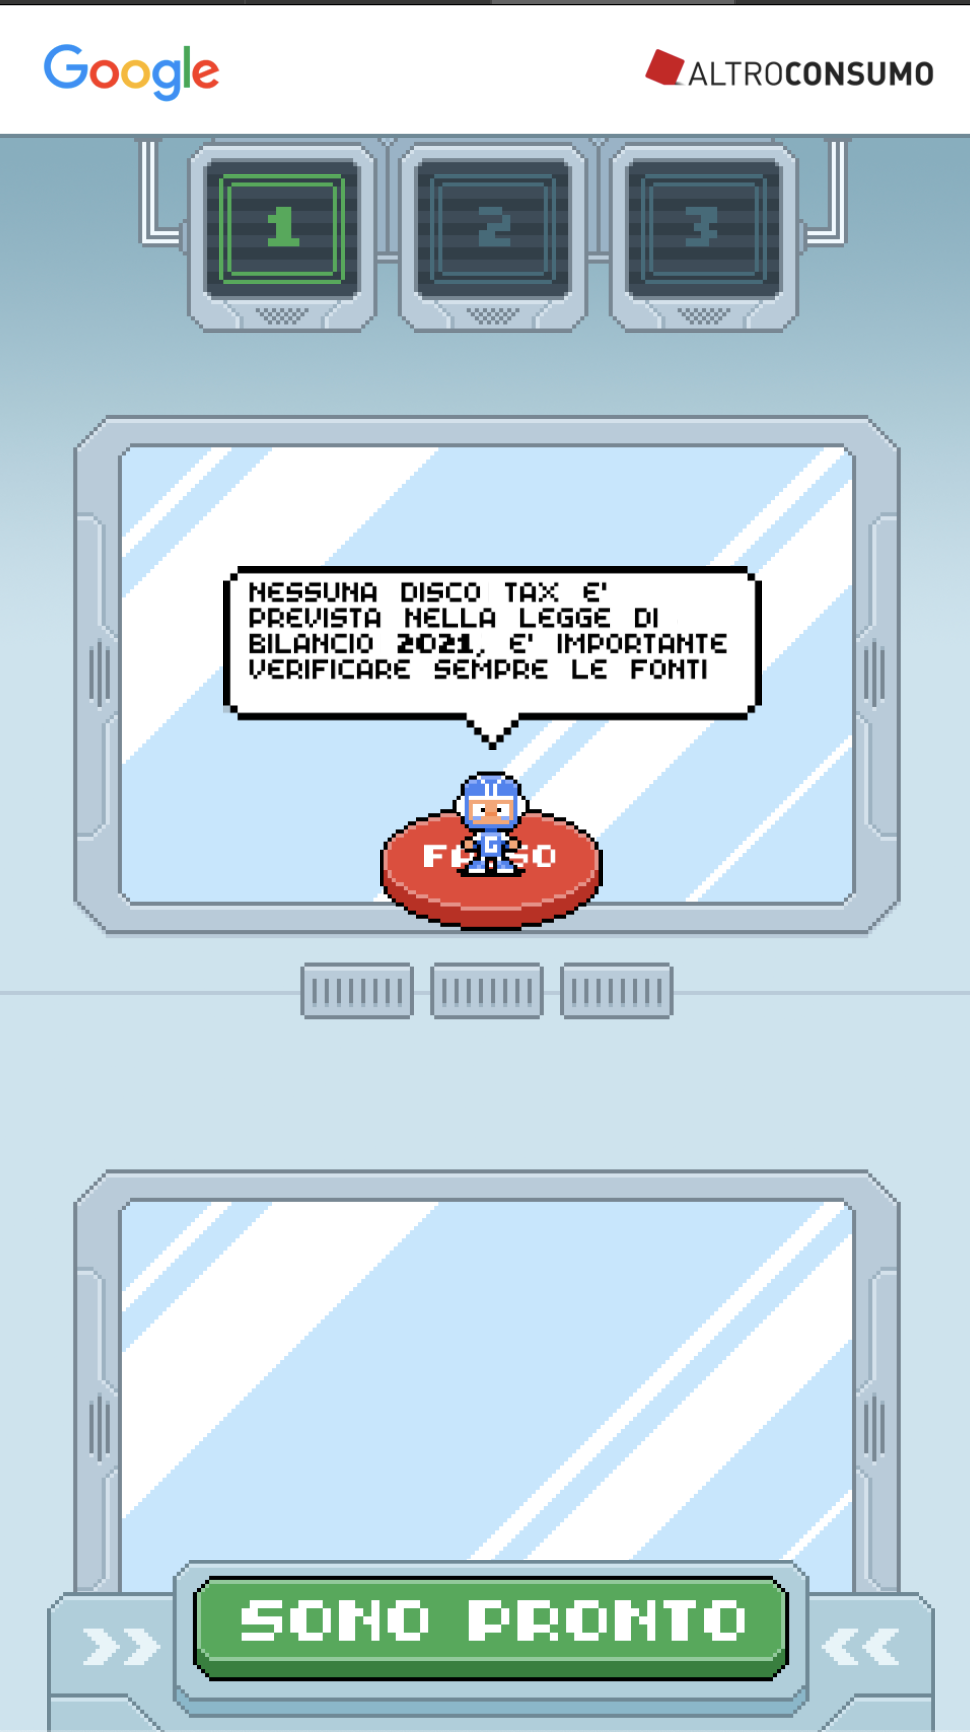
\includegraphics[width=0.30\textwidth]{img/infoTower3.png}
    }
    \caption{Information Tower: serious game per imparare a distinguere le \textit{fake news}}
    \label{fig:infoTower}
\end{figure}

\subsubsection{Minecraft Education Edition - Educazione scolastica}
Questa versione del noto gioco Minecraft \cite{minecraftEdu} permette d'insegnare utilizzando un gioco familiare agli alunni rendendo meno noioso e divertente l'apprendimento. Sono disponibili gratuitamente tantissime mappe che spaziano su diversi argomenti. Un modo d'insegnare che anche assomiglia all'utilizzo della realtà virtuale.

\begin{figure}
    \center
    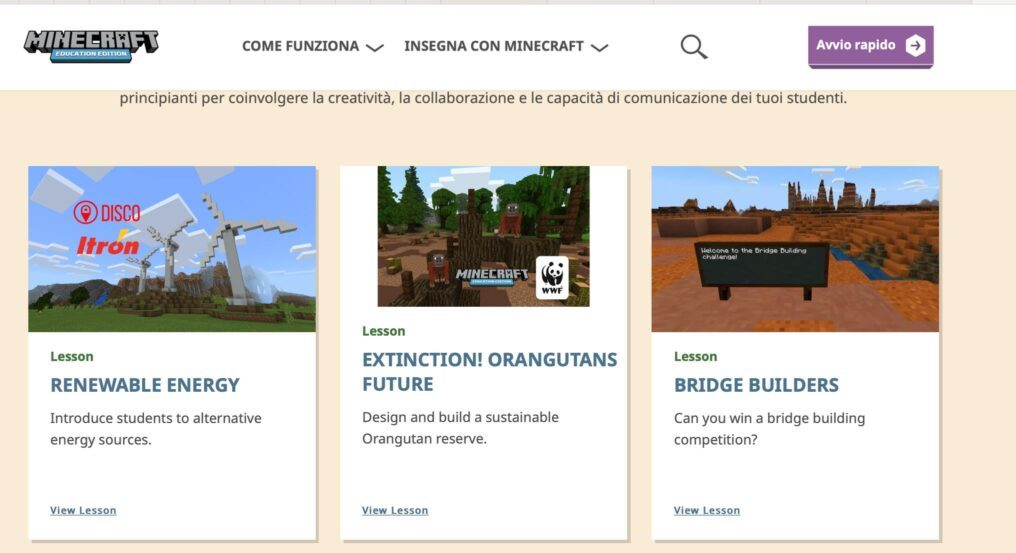
\includegraphics[width=0.70\textwidth]{img/minecraft-lessons.jpg}
    \caption{Minecraft Education: alcune lezioni proposte sul sito ufficiale}
    \label{fig:minecraftEdu}
\end{figure}

\subsubsection{Spent - Sensibilizzazione e raccolta fondi}
Spent \cite{spentGame} è un gioco pensato per stimolare le donazioni in aiuto delle persone con basso reddito o in stato di povertà. Questo gioco cerca di  sviluppare empatia e comprensione per queste persone portando il giocatore a dover fare scelte economiche, personali e lavorative molto difficili in modo da superare i 30 livelli nonché giorni presenti tipicamente in un mese.
Alla fine del gioco viene chiesto di fare una offerta.

\begin{figure}
    \center
    \subfloat[Schermata iniziale dove l'utente viene sfidato]{
        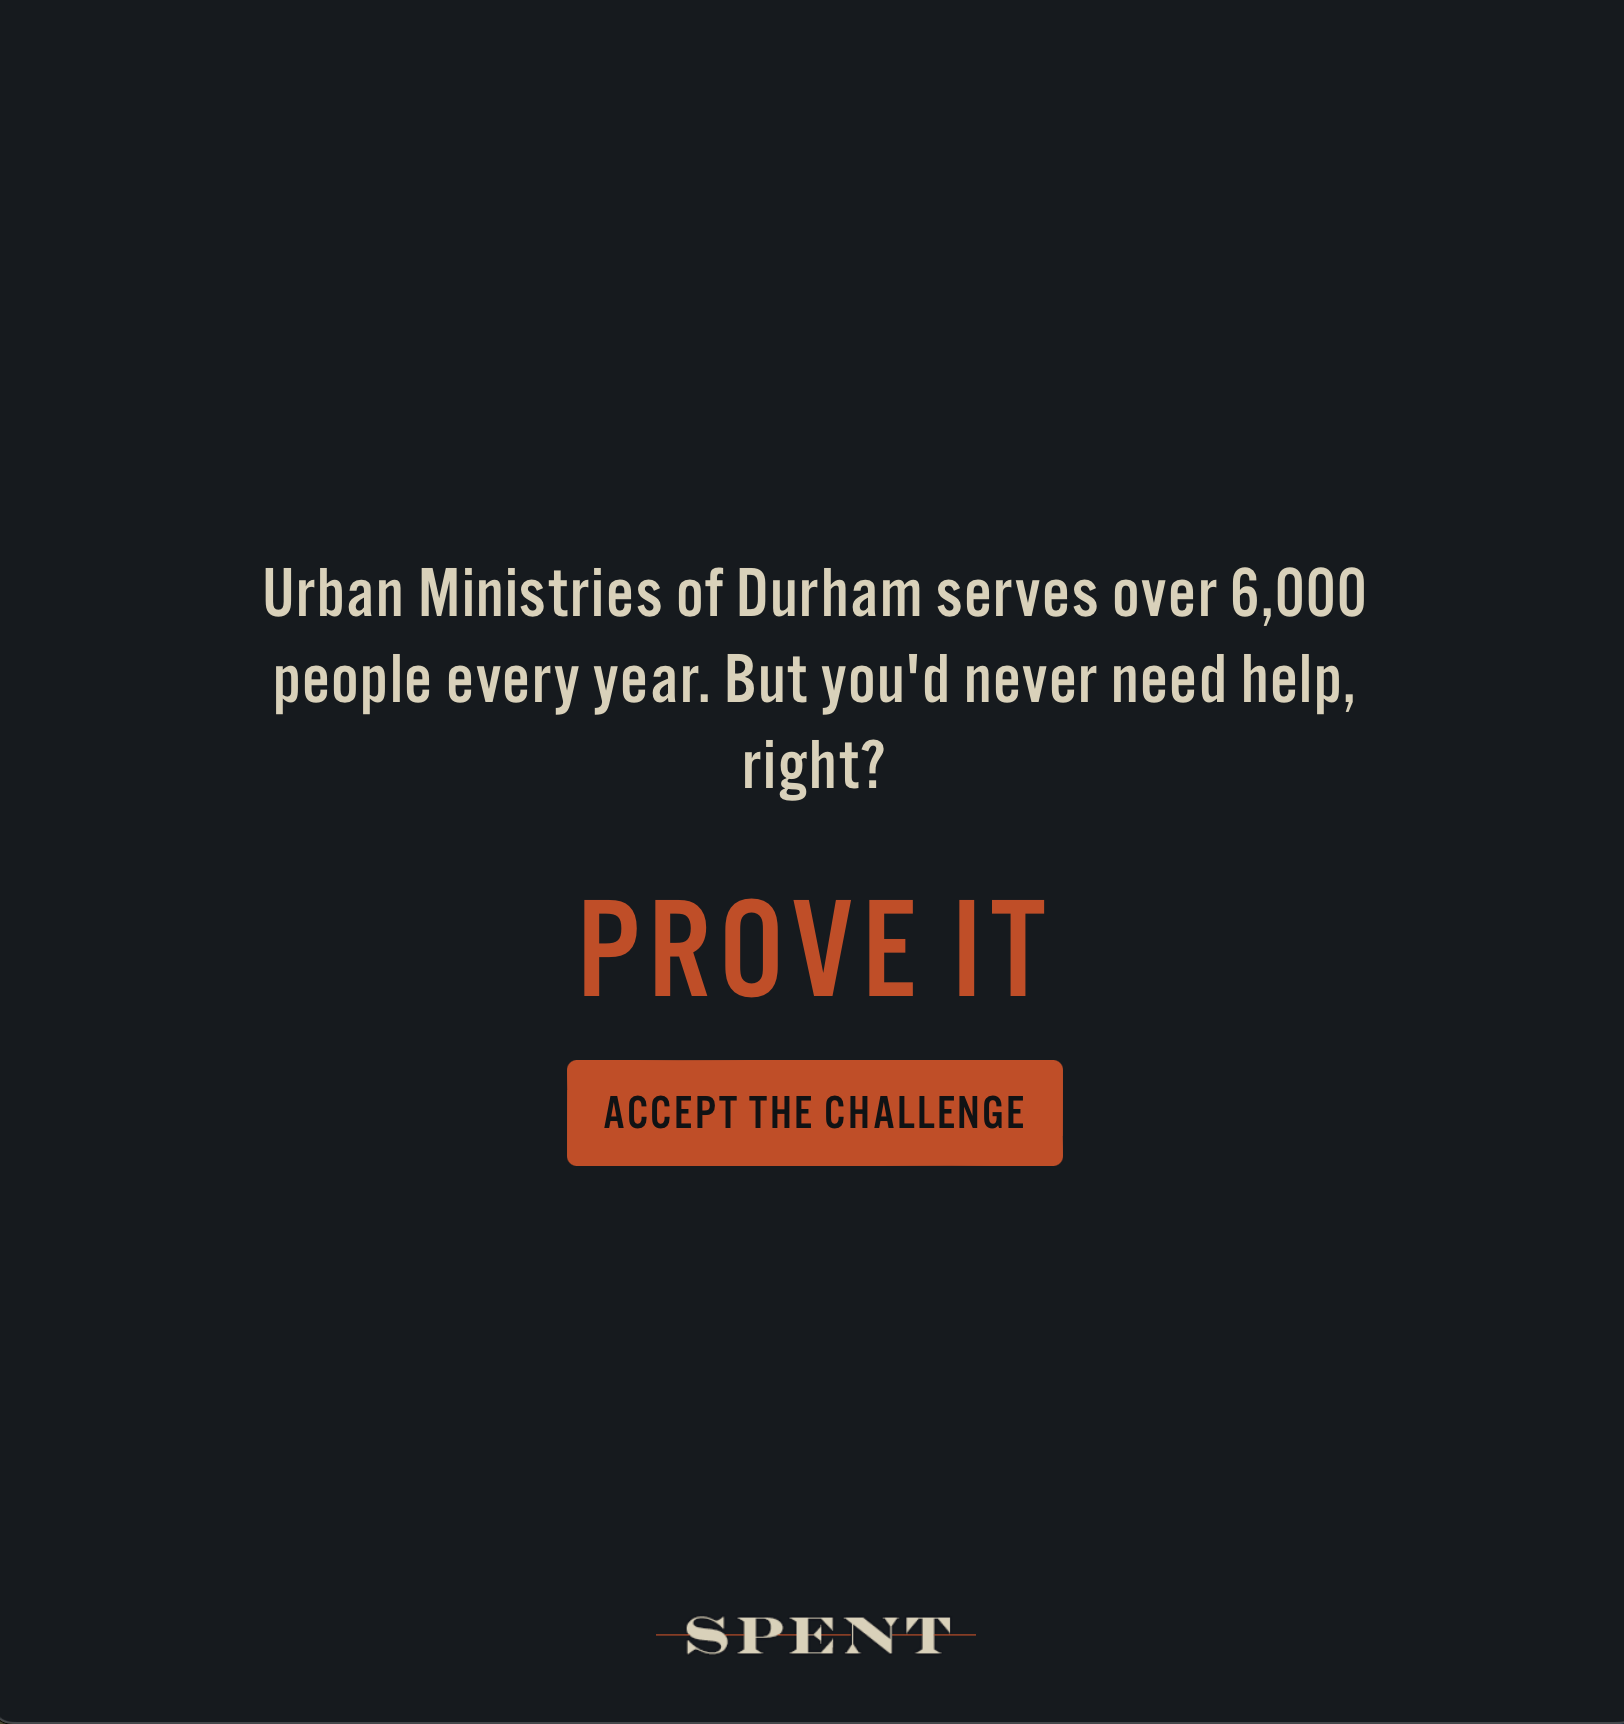
\includegraphics[width=0.45\textwidth]{img/spent1.png}
    }
    \subfloat[Primo giorno di povertà, prima scelta da fare]{
        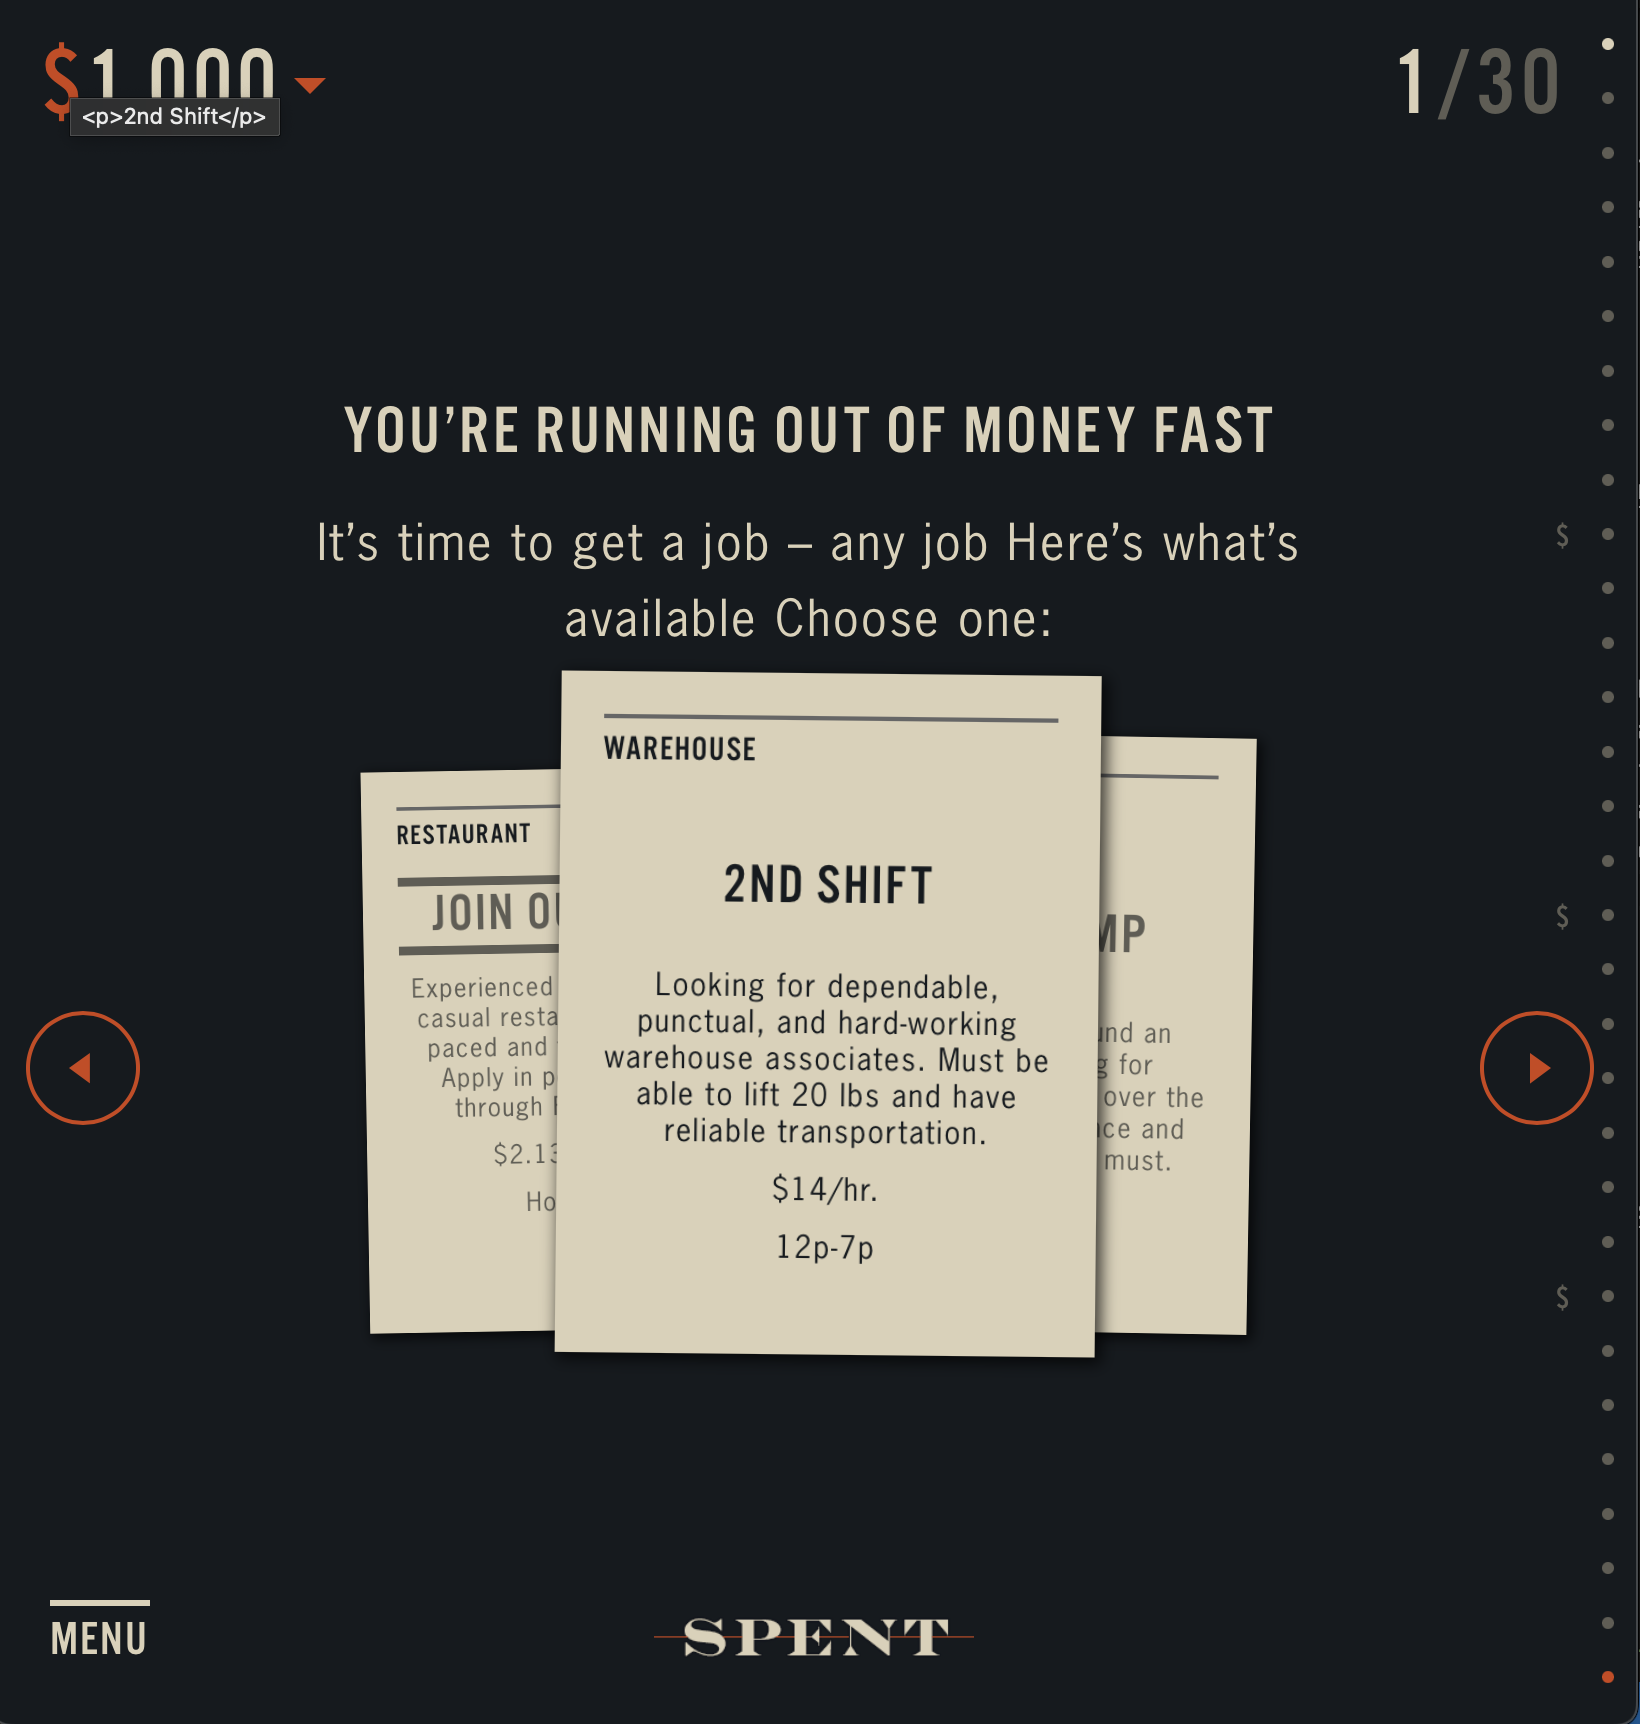
\includegraphics[width=0.45\textwidth]{img/spent2.png}
    }
    \caption{Spent: serious game di sensibilizzazione e raccolta fondi per persone a basso reddito}
    \label{fig:spentGame}
\end{figure}
%
\section{Extended Reality}
Extended Reality (XR), in italiano Realtà Estesa, è un termine che raggruppa tutte le possibili realtà che si possono generare utilizzando sistemi elettronici e informatici per portare una o più persone in realtà potenziate o totalmente generate dal computer.
Si identificano tre tipologie:

\begin{itemize}
    \item \textbf{Realtà Aumentata (AR)}: l'ambiente reale circostante viene integrato con oggetti virtuali e/o informazioni utili aggiunti digitalmente;
    \item \textbf{Realtà Virtuale (VR)}: la realtà circostante viene completamente sostituita con una virtuale;
    \item \textbf{Realtà Mista (MR)}: il mondo reale e la realtà virtuale coesistono in una unica realtà
\end{itemize}

Per poter di utilizzare e sfruttare le potenzialità di queste realtà, sono disponibili sul mercato svariate tecnologie hardware e software. Di seguito un elenco, probabilmente non esaustivo:

\begin{itemize}[]
    \itemsep0.5em
    \item \textit{Head-Mounted Devices} (HMDs), dispositivi da mettere sulla testa, comprendente di visore, che grazie ai sensori e alle videocamere presenti, le interazioni possono avvenire usando il movimento della testa (\textit{Hand-free}), con controller oppure  attraverso le proprie mani senza la necessita di ulteriori dispositivi;
    \item Smartphone e tablet, attraverso lo schermo e grazie alla videocamera e i sensori è possibile utilizzare l'AR;
    \item Smart Glasses, occhiali per l'AR che permettono di visualizzare informazioni di ogni genere anche contestuali a ciò che si sta guardando.
    \item Tute e guanti aptici, per la realtà virtuale, che permettono di trasmettere sensazioni tattili, tracciare il movimento del corpo e i dati biometrici e gestire la temperatura rendendo l'esperienza virtuale il più reale possibile;
    \item Tapis roulant per simulare il movimento nel mondo in VR;
    \item Cuffie o auricolari per simulare o integrare la sfera sonora dell'utente grazie all'audio spaziale.
\end{itemize}

\subsection{Realtà aumentata}
\label{sec:ar}
La Realtà Aumentata (in inglese Augmented Reality, AR) consiste nell'arricchire il mondo reale circostante con oggetti e informazioni multimediali di vario genere e tipologia che normalmente non sarebbero percepibili dai cinque sensi.
In una indagine condotta su dieci esperti del settore, accademici e industriali, è risultato che per alcuni si parla già di realtà aumentata con semplici sovrapposizioni d'informazioni attinenti al contesto in cui l'utente si trova mentre, per altri, si ritiene necessaria una registrazione spaziale e/o una interazione con lo spazio circostante \cite[ Capitolo 4, What is AR?]{whatMR}.

Questi arricchimenti sono fruibili per mezzo di dispositivi come ad esempio visori AR, computer provvisti di webcam, smartphone, auricolari, lenti a contatto o tecniche particolari come il Video Mapping che fa uso di proiezioni sulle superfici e oggetti senza la necessità d'indossare alcun dispositivo (Spatially Argumented Reality \cite{Raskar1999SpatiallyAR}).

Si identificano tre tipologie di AR che si differenziano in base al criterio utilizzato per il posizionamento degli elementi \enquote{aumentanti} nell'ambiente circostante; si hanno quindi Realtà Aumentate:

\begin{description}
    \itemsep1em
    \item \textbf{\textit{Location-based}} (Figura \ref{fig:location_ar}), dove gli elementi vengono disposti in una precisa posizione geografica GPS, ad esempio viene mostrata una icona in corrispondenza di punti d'interesse (POI) in tempo reale, o per esempio può essere emesso un suono specifico in corrispondenza di uno di questi;
    \item \textbf{\textit{Marker-based}} (Figura \ref{fig:marker_ar}), gli oggetti vengono sovrapposti e posizionati sul marker che può essere un codice QR, una immagine o un disegno;
    \item \textbf{\textit{Markerless}} (Figura \ref{fig:markerless_ar}), dopo una scansione dell'ambiente circostante, ad esempio con la fotocamera dello smartphone, gli oggetti vengono collocati su quelle caratteristiche ambientali ritenute adatte (es. superfici orizzontali, verticali, o particolari come ad esempio un viso umano). Un esempio caratteristico sono i filtri di Instagram che aggiungono e modificano la percezione della nostra faccia con maschere, strucchi od oggetti (Figura \ref{fig:instaFilter}).
    \begin{figure}
        \centering
        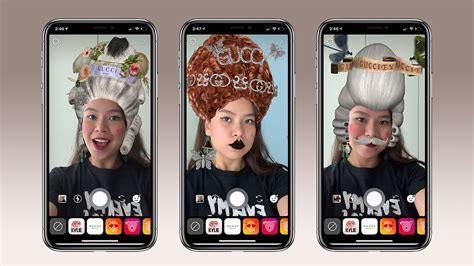
\includegraphics[width=0.5\textwidth]{img/instaFilter.jpeg}
        \caption{Filtri di Instagram come esempio di realtà aumentata \textit{markerkless} su superfici non regolari}
        \label{fig:instaFilter}
    \end{figure}
\end{description}

\begin{figure}
    \centering
    \subfloat[Funzionalità Live View in Google Maps che utilizza l'AR Location-based]{
        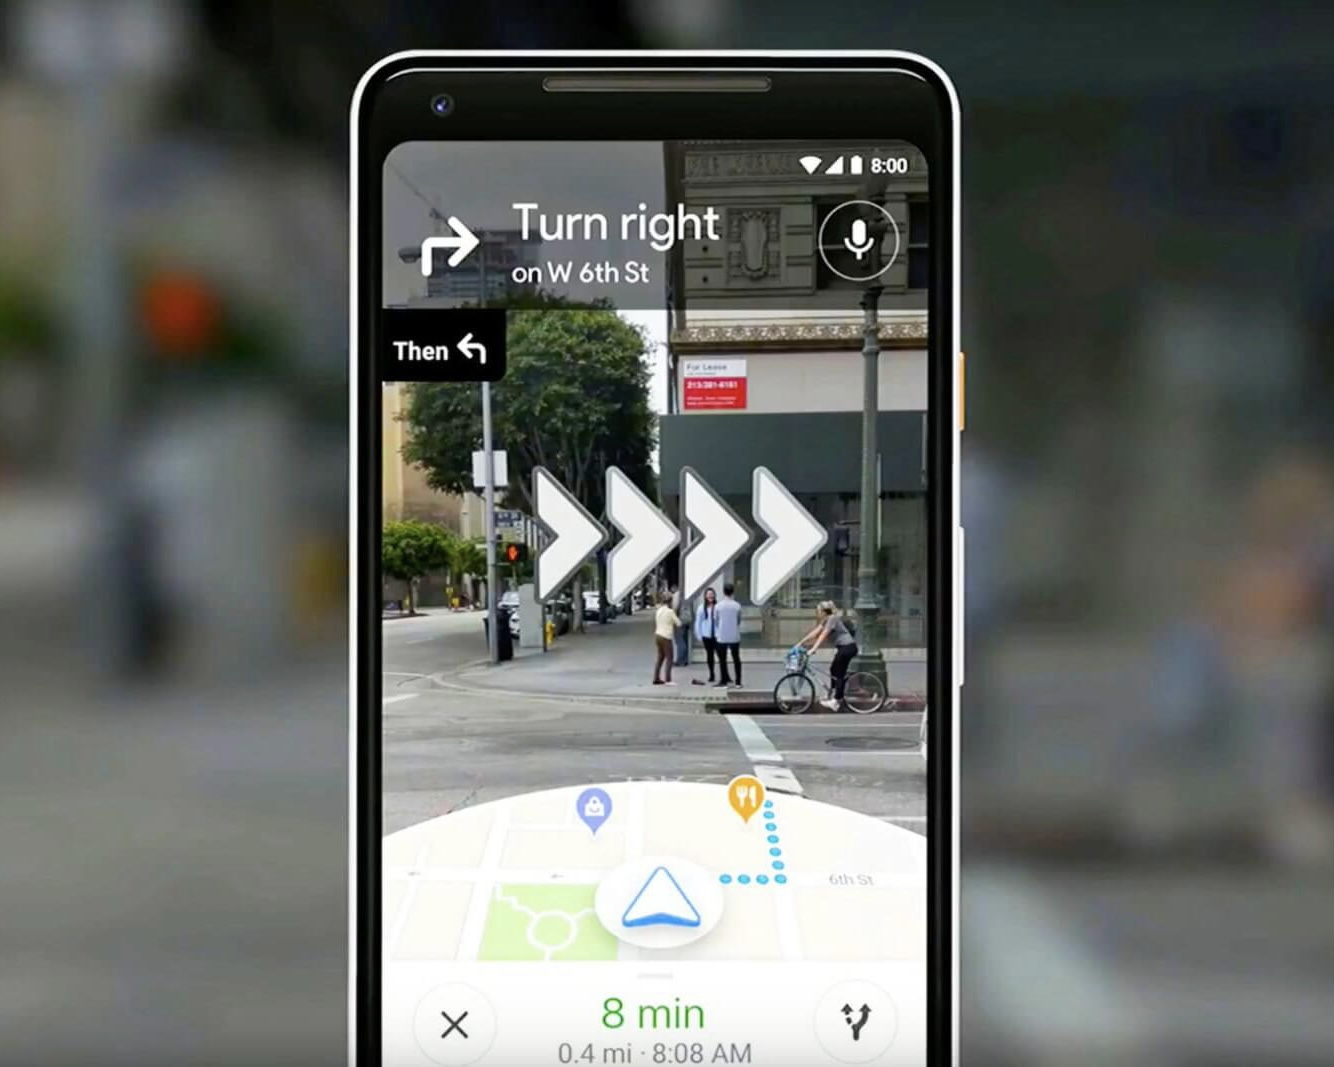
\includegraphics[width=0.32\textwidth]{img/location-based-ar.jpg}
        \label{fig:location_ar}
    }
    \subfloat[Marker-based AR]{
        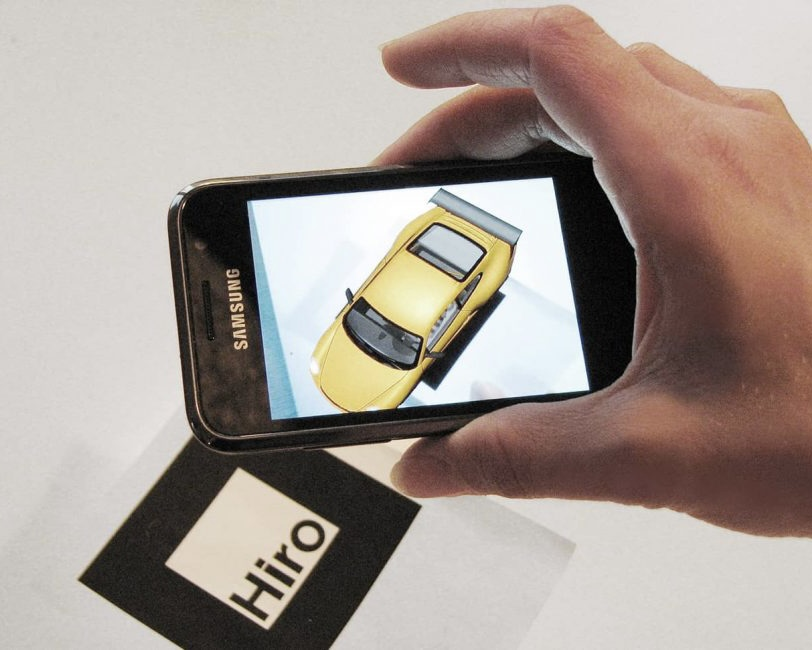
\includegraphics[width=0.32\textwidth]{img/marker-base-ar.jpg}
        \label{fig:marker_ar}
    }
    \subfloat[Markerless AR: App IKEA Place]{
        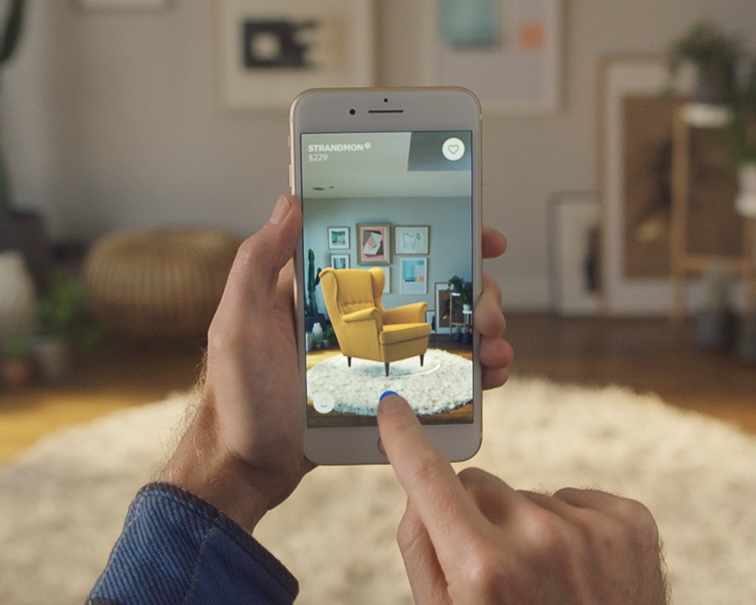
\includegraphics[width=0.32\textwidth]{img/markerless-ar.jpg}
        \label{fig:markerless_ar}
    }
    \caption{Esempi di tre tipologie di Realtà Aumentata} 
    \label{fig:ARbased_type}
\end{figure}

\subsection{Realtà Virtuale}
La Realtà Virtuale (in inglese Virtual Reality, VR) rimpiazza l'ambiente circostante con uno che può realmente esistere (es. simulazioni) o completamente virtuale (es. videogichi), isolando l'utente da tutte le interazioni sociali esterne reali.

Si usa tipicamente un visore VR per la generazione di un ambiente virtuale con l'ausilio di dispositivi come tute, guanti, maschere o cuffie per rendere più immersiva e realistica l'esperienza virtuale ma, come nel caso delle simulazioni di volo, l'ambiente può anche essere proiettato su pareti e la plancia di comando essere vera (in questo caso si potrebbe ricadere in una mixed reality in cui la cabina dell'aereo vera, la realtà, si mescola con la pista e il cielo virtuali).

Oltre a essere impiegata dall'industria dei videogiochi ha trovato una ottima applicazione insieme ai \textit{serious game} in attività formative scolastiche, di ricerca, mediche e terapeutiche (es. trattamento ustioni).

Sono presenti molte ricerche che dimostrano o studiano l'efficacia di questa tecnologia nell'apprendimento e nella formazione. Fra questi si cita l'articolo \citetitle{HMDmedicalSeriousgame}\cite{HMDmedicalSeriousgame} che mette in evidenza come, nelle simulazioni di operazioni chirurgiche, su un totale di 27 studi condotti con 956 partecipanti, solo 2 (il 7\%) non hanno avuto benefici dall'impiego di AR/VR basati su Head Mounted Devices.

\subsubsection{Snow World - Terapia VR per il dolore da ustioni}
Si tratta di \textit{Virtual-Reality therapy} e si cita lo studio condotto da Hoffman e Paterson nella Università di Washington, Seattle e del centro ustioni Harborview Burn Center \cite{vrpain}, dove viene utilizzata la realtà virtuale, con il gioco Snow World (Figura \ref{fig:snowworld}), per distrarre i pazienti, con gravi ustioni, dal dolore durante i trattamenti giornalieri come il cambio delle bende, pulizia delle ferite e la rimozione delle graffette.

\begin{figure}
    \centering
    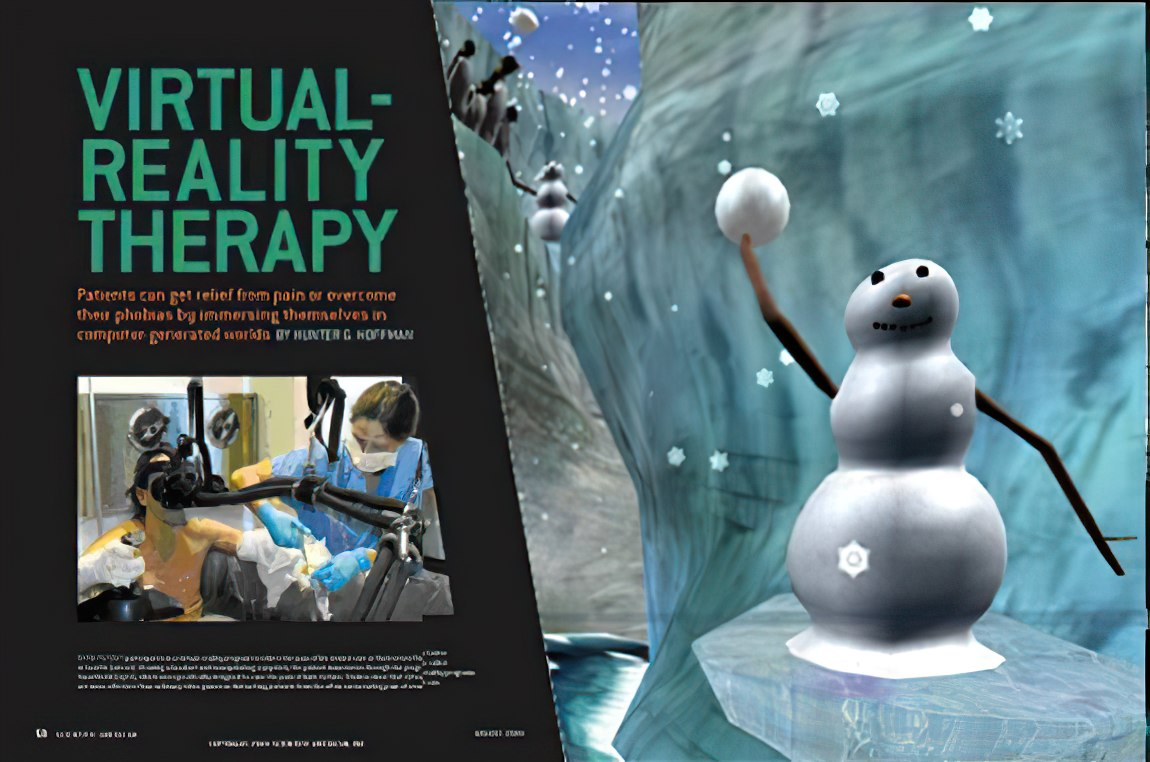
\includegraphics[width=0.7\textwidth]{img/snowworld.jpg}
    \caption{Snow World: terapia in VR per il trattamento di ustioni}
    \label{fig:snowworld}
\end{figure}

\subsection{Mixed reality}
La mixed reality viene descritta nella letteratura come uno spettro della realtà dove a un estremo c'è il mondo reale e in quell'altro estremo c'è la realtà virtuale, tutte le realtà in mezzo sono parte della realtà mista. Quindi possiamo trovare secondo questa definizione, la realtà aumentata che si trova all'interno di questo spettro così come per quella virtuale.
%TODO FINIRE
MR is a highly interdisciplinary field engaging signal processing, computer vision, computer graphics, user interfaces, human factors, wearable computing, mobile computing, information visualization, and the design of displays and sensors. 
In MR systems, users perceive both the physical environment around them and digital elements presented through, for example, the use of semitransparent displays.
MR systems are designed to give their users the illusion that digital objects are in the same space as physical ones (Figure 1). For this illusion of coexistence, the digital objects need to be precisely positioned into the real environment and aligned with the real objects in real time
Augmented reality is often considered to be a branch of MR. (Mixed reality.pdf)

%
%
\section{Integrazione tra diversi tipi di device}
In sistemi che presentano vari dispositivi, che potrebbero anche utilizzare tecnologie diverse, molto spesso è richiesta la loro comunicazione e collaborazione per assolvere uno o più compiti.
Come primo passo occorre considerare diversi aspetti del sistema, come per esempio la quantità d'informazioni da condividere tra i \textit{device}, la loro distanza, le tecnologie hardware a disposizione, l'aspetto della sicurezza o la velocità di comunicazione.

Una prima scelta può essere fatta in base alle tecnologie hardware e protocolli disponibili sui device, di seguito le principali:
%TODO FINIRE
\begin{itemize}
    \item Wireless {
        \begin{itemize}
        \item Bluetooth
        \item NFC (Near Field Communication)
        \item Beacon (funziona con tecnologia Bluetooth Low Energy) usati in Proximity Marketing
        \end{itemize}
        }
    \item Wired (cablato, marea di protocolli di trasmissione) sicuramente affidabile e veloce ma poco pratico se si hanno dispositivi mobili
    
\end{itemize}

mentre, a un più alto livello di astrazione, si hanno a disposizione diverse alternative tra cui:

\begin{itemize}
    \item \textit{Application Programming Interface API}
    \item \textit{Middleware}
    \item \textit{Cloud computing}
    \item \textit{Web services}
    \item \textit{Service-oriented architecture}
\end{itemize}

\section{Integrazione tra totem e smartphone}
L'integrazione fra totem e smartphone ha richiesto un'analisi sulla disponibilità e praticabilità di utilizzare determinate tecnologie per l'interazione fra i due dispositivi anche in un'ottica di user experience, usabilità e scalabilità.

Per questo progetto si è optato per una integrazione che utilizza il \textit{cloud computing} e più precisamente utilizzando un servizio \textit{cloud-based} per la memorizzazione in tempo reale dei dati; viene utilizzato il prodotto Firebase Realtime di Google \cite{firebase} in un'ottica anche di scalabilità, affidabilità, facilità d'uso e sicurezza.
Scegliendo questo modo d'integrazione si apre la possibilità di aggiungere nuove postazioni interattive (totem) nel tempo in caso di diffusione di questo progetto anche in altre sedi.

Si è valutato l'utilizzo della tecnologia NFC per il trasferimento dei dati da APP a totem interattivo ma la mancanza dell'hardware necessario e considerato che non tutti gli smartphone (in particolare quelli meno recenti) possiedono tale tecnologia si è deciso di non utilizzarla.

Come ulteriore alternativa si è valutato l'utilizzo di una architettura client-server, connessi alla stessa rete locale, utilizzando delle API messe a disposizione dal web-server, all'interno del totem, per il caricamento dei dati da parte dell'APP. Quest'ultima opzione poteva essere buona in termini di sicurezza e velocità di trasmissione ma poco scalabile e avrebbe circoscritto la condivisione dei dati a solo quegli utenti connessi alla rete dell'Ateneo in sede a Cesena.